% -*- latex -*-
%%%%%%%%%%%%%%%%%%%%%%%%%%%%%%%%%%%%%%%%%%%%%%%%%%%%%%%%%%%%%%%%
%%%%%%%%%%%%%%%%%%%%%%%%%%%%%%%%%%%%%%%%%%%%%%%%%%%%%%%%%%%%%%%%
%%%%
%%%% This text file is part of the source of slides for
%%%% `The Art of HPC, vol 1: The Science of Computing'
%%%% by Victor Eijkhout, copyright 2012-2022
%%%%
%%%%%%%%%%%%%%%%%%%%%%%%%%%%%%%%%%%%%%%%%%%%%%%%%%%%%%%%%%%%%%%%
%%%%%%%%%%%%%%%%%%%%%%%%%%%%%%%%%%%%%%%%%%%%%%%%%%%%%%%%%%%%%%%%


\frame{\frametitle{Sparse matrix storage}

 Matrix above has many zeros: $n^2$ elements but only $O(n)$
  nonzeros. Big waste of space to store this as square array.

 Matrix is called  `sparse' if there are enough zeros to make
  specialized storage feasible.

  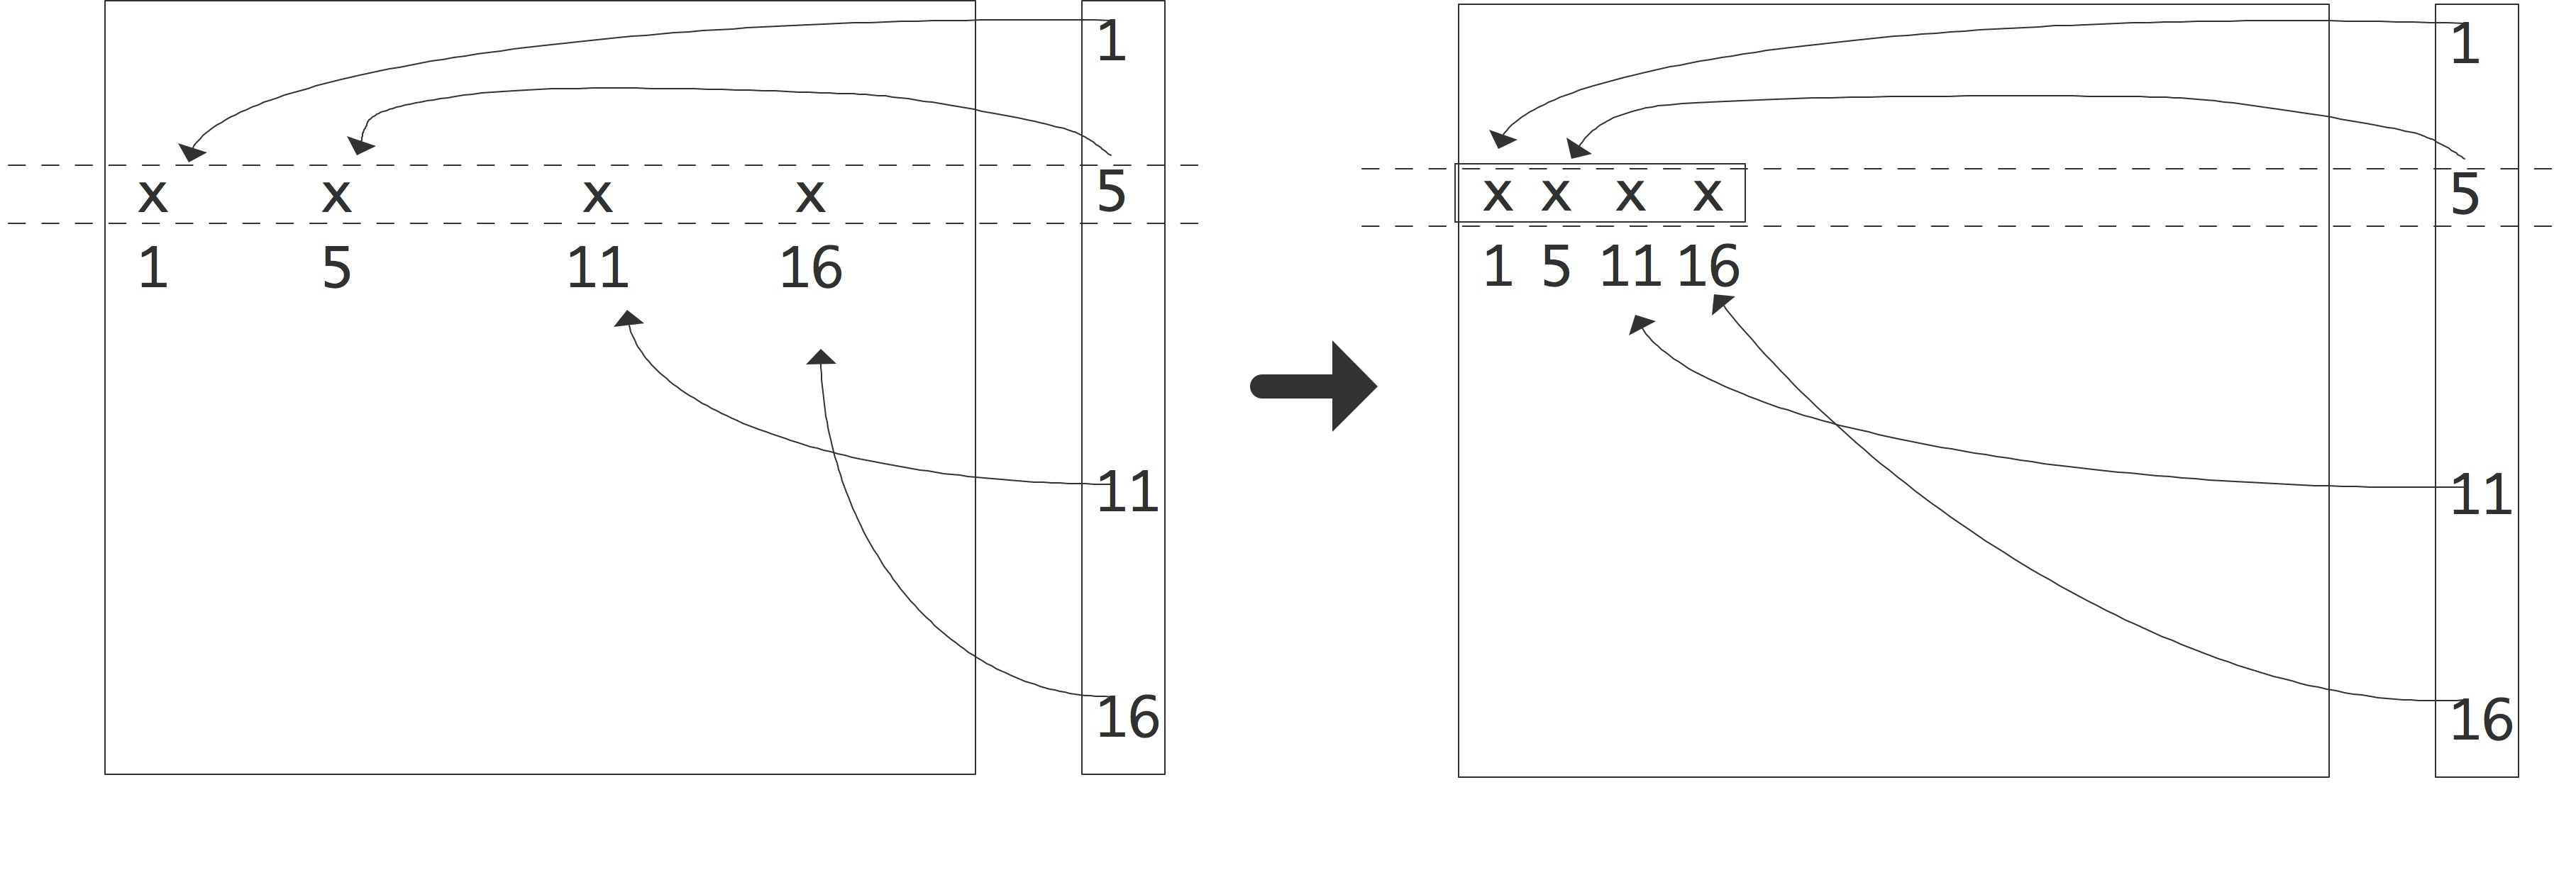
\includegraphics[scale=.08]{crs}
}


\frame{\frametitle{Compressed Row Storage}
\begin{equation}
A =
\left(\begin{array}{rrrrrr}
      10 &  0 &  0 & 0  &-2 &  0 \\
       3 &  9 &  0 & 0  & 0 &  3 \\
       0 &  7 &  8 & 7  & 0 &  0 \\
       3 &  0 &  8 & 7  & 5 &  0 \\
       0 &  8 &  0 & 9  & 9 & 13 \\
       0 &  4 &  0 & 0  & 2 & -1
           \end{array}
\right) ~.
\end{equation}
 Compressed Row Storage (CRS): store all nonzeros by row, their column
  indices, pointers to where the columns start (1-based indexing):
\begin{center}
\begin{tabular}{|r|r|r|r|r|r|r|r|r|r|r|r|r|r|r|r|} \hline
{\tt val}     &10 &-2& 3& 9& 3& 7& 8& 7& 3 $\cdots$  9&13& 4& 2&-1 \\ \hline
{\tt col\_ind}& 1 & 5& 1& 2& 6& 2& 3& 4& 1 $\cdots$  5& 6& 2& 5& 6 \\ \hline
\end{tabular} \\
\vspace{.02 in}
\begin{tabular}{|r|r|r|r|r|r|r|r|} \hline
{\tt row\_ptr}& 1 & 3 & 6 & 9 & 13 & 17 & 20  \\ \hline
\end{tabular} ~.
\end{center}
}

% \frame{\frametitle{Band matrix storage}

%  Matrix from 5-point stencil is a band matrix:
% \[ \exists_{p,q\geq0}\colon (j<i-p\vee j>i+q)\rightarrow a_{ij}=0 \]
% }

\begin{frame}{Sparse matrix-vector operations}
  \begin{itemize}
  \item Simplest, and important in many contexts: matrix-vector product.
  \item Matrix-matrix product rare in engineering science\\
    very important in Deep Learning
  \item Gaussian elimination is a complicated story.
  \item In general: changes to sparse structure are hard!
  \end{itemize}
\end{frame}

\frame[containsverbatim]{\frametitle{Dense matrix-vector product}
  Most common operation in many cases: matrix-vector product
\begin{verbatim}
aptr = 0;
for (row=0; row<nrows; row++) {
   s = 0;
   for (col=0; col<ncols; col++) {
      s += a[aptr] * x[col];
      aptr++;
   }
   y[row] = s;
}
\end{verbatim}
Reuse? Locality? Cachelines?
}

\begin{frame}{Better implementation}
  Three loops: block, columns inside block, row;\\
  permute blocks to outermost

  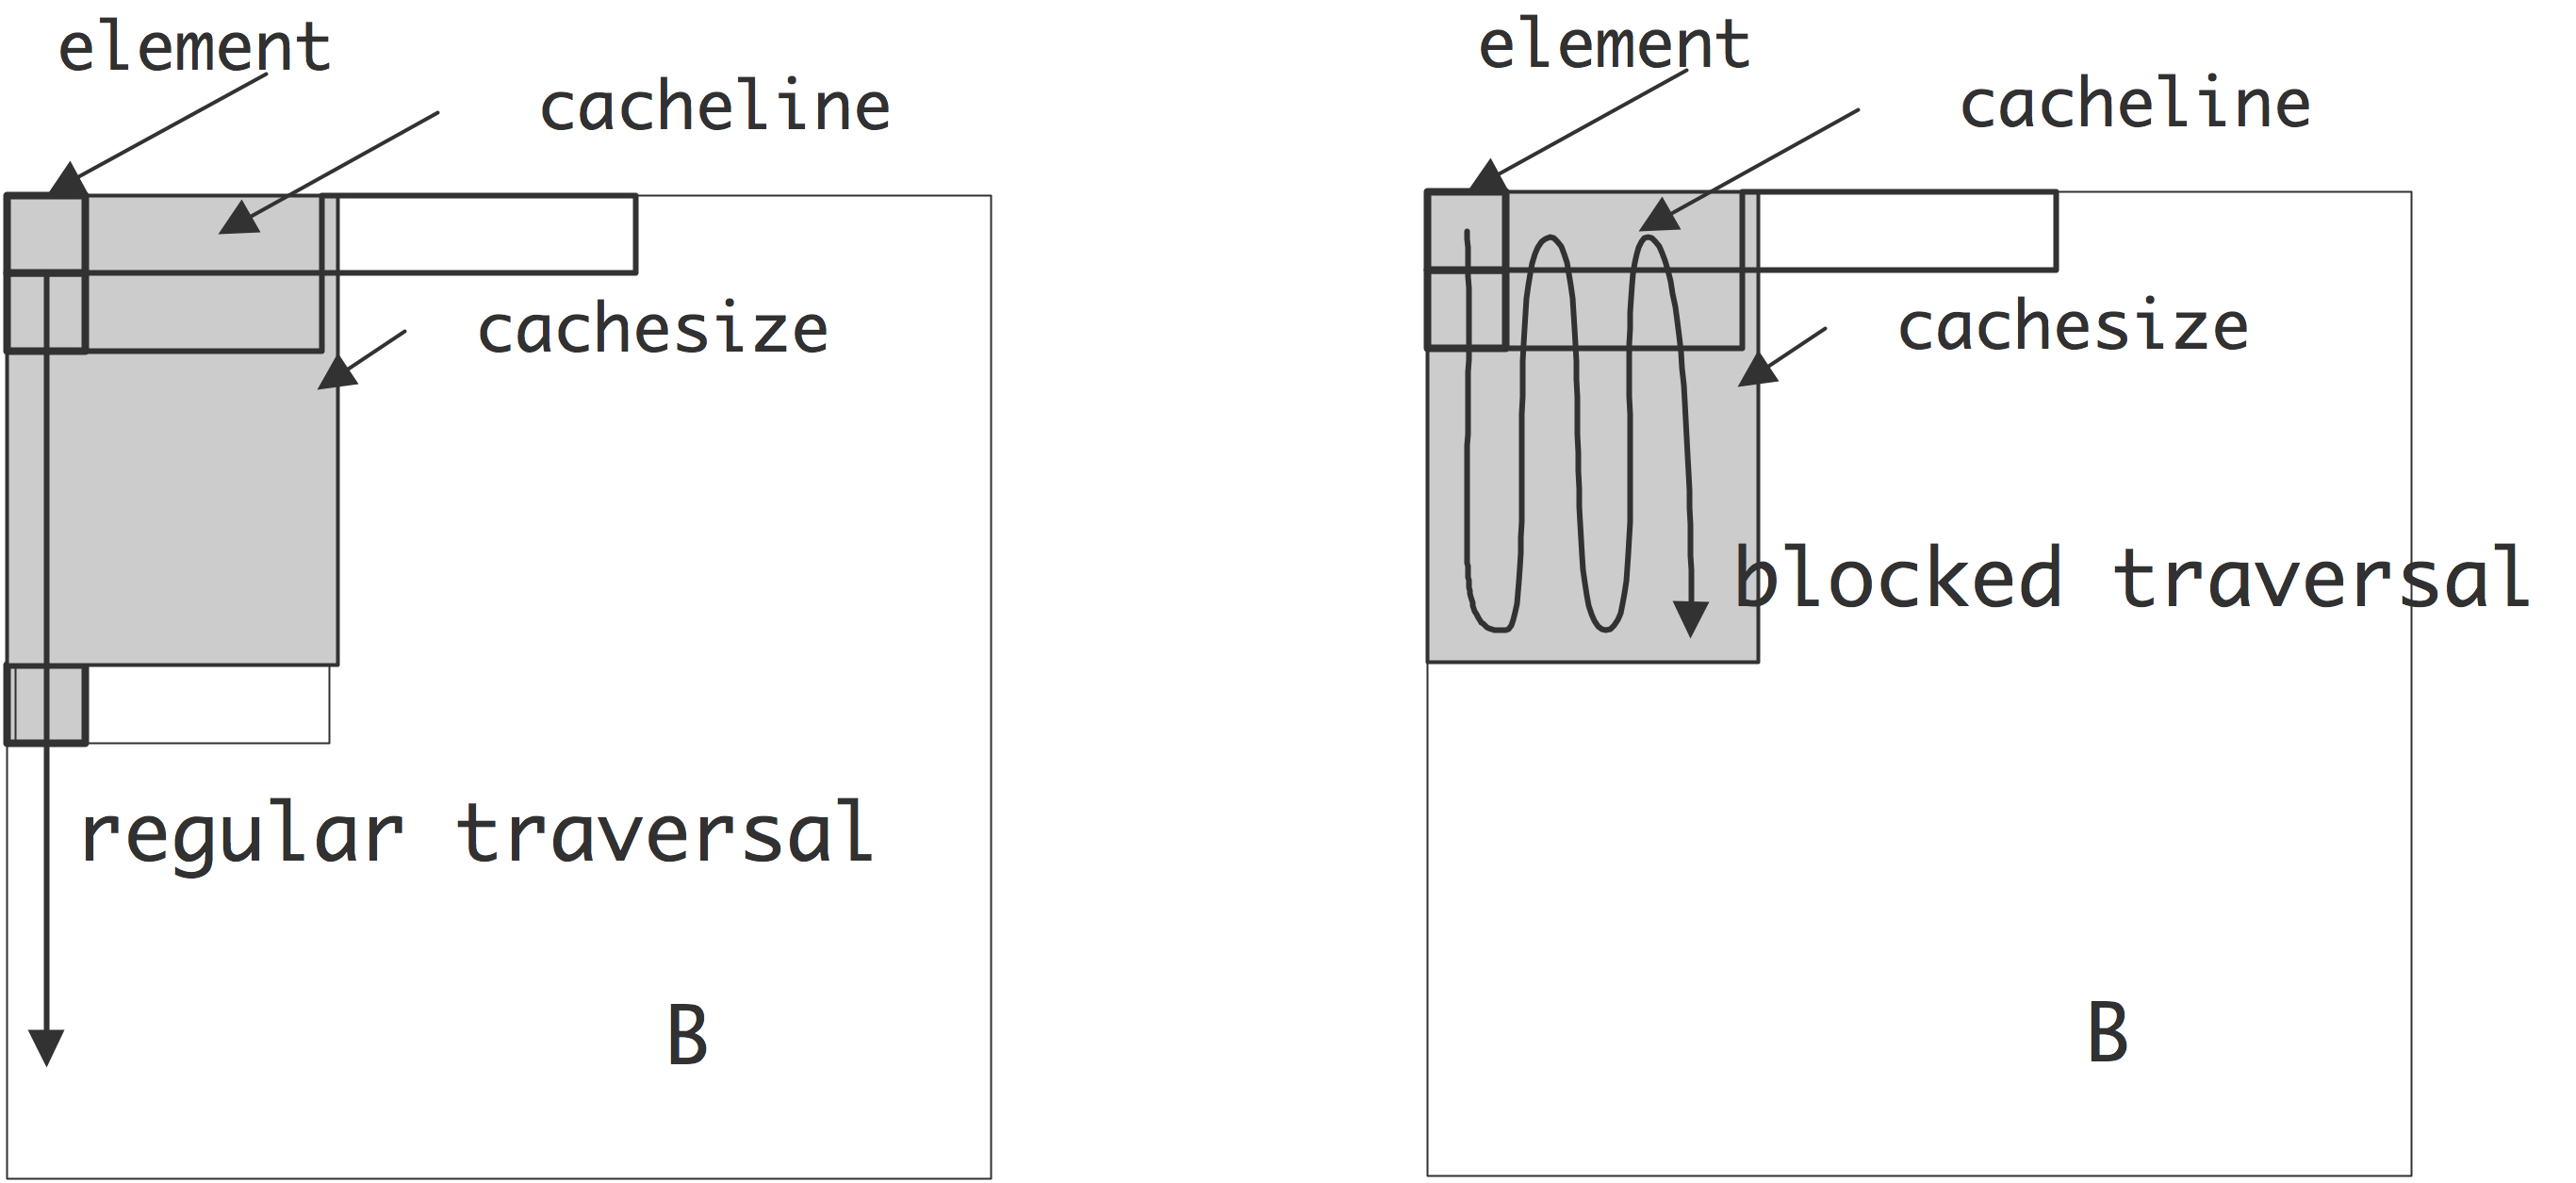
\includegraphics[scale=.12]{blockedtranspose}
\end{frame}

\frame[containsverbatim]{\frametitle{Sparse matrix-vector product}
\begin{verbatim}
aptr = 0;
for (row=0; row<nrows; row++) {
   s = 0;
   for (icol=ptr[row]; icol<ptr[row+1]; icol++) {
      int col = ind[icol];
      s += a[aptr] * x[col];
      aptr++;
   }
   y[row] = s;
}
\end{verbatim}
Again: Reuse? Locality? Cachelines?

Indirect addressing of \texttt{x} gives low spatial and temporal locality.
}

\begin{frame}{Exercise: sparse coding}
  What if you need access to both rows and columns at the same time?
  Implement an algorithm that tests whether a matrix stored in CRS
  format is symmetric. Hint: keep an array of pointers, one for each
  row, that keeps track of how far you have progressed in that row.
\end{frame}

\begin{diagonalstorage}
  \begin{frame}{Storage by diagonals}
    Use the banded format:

    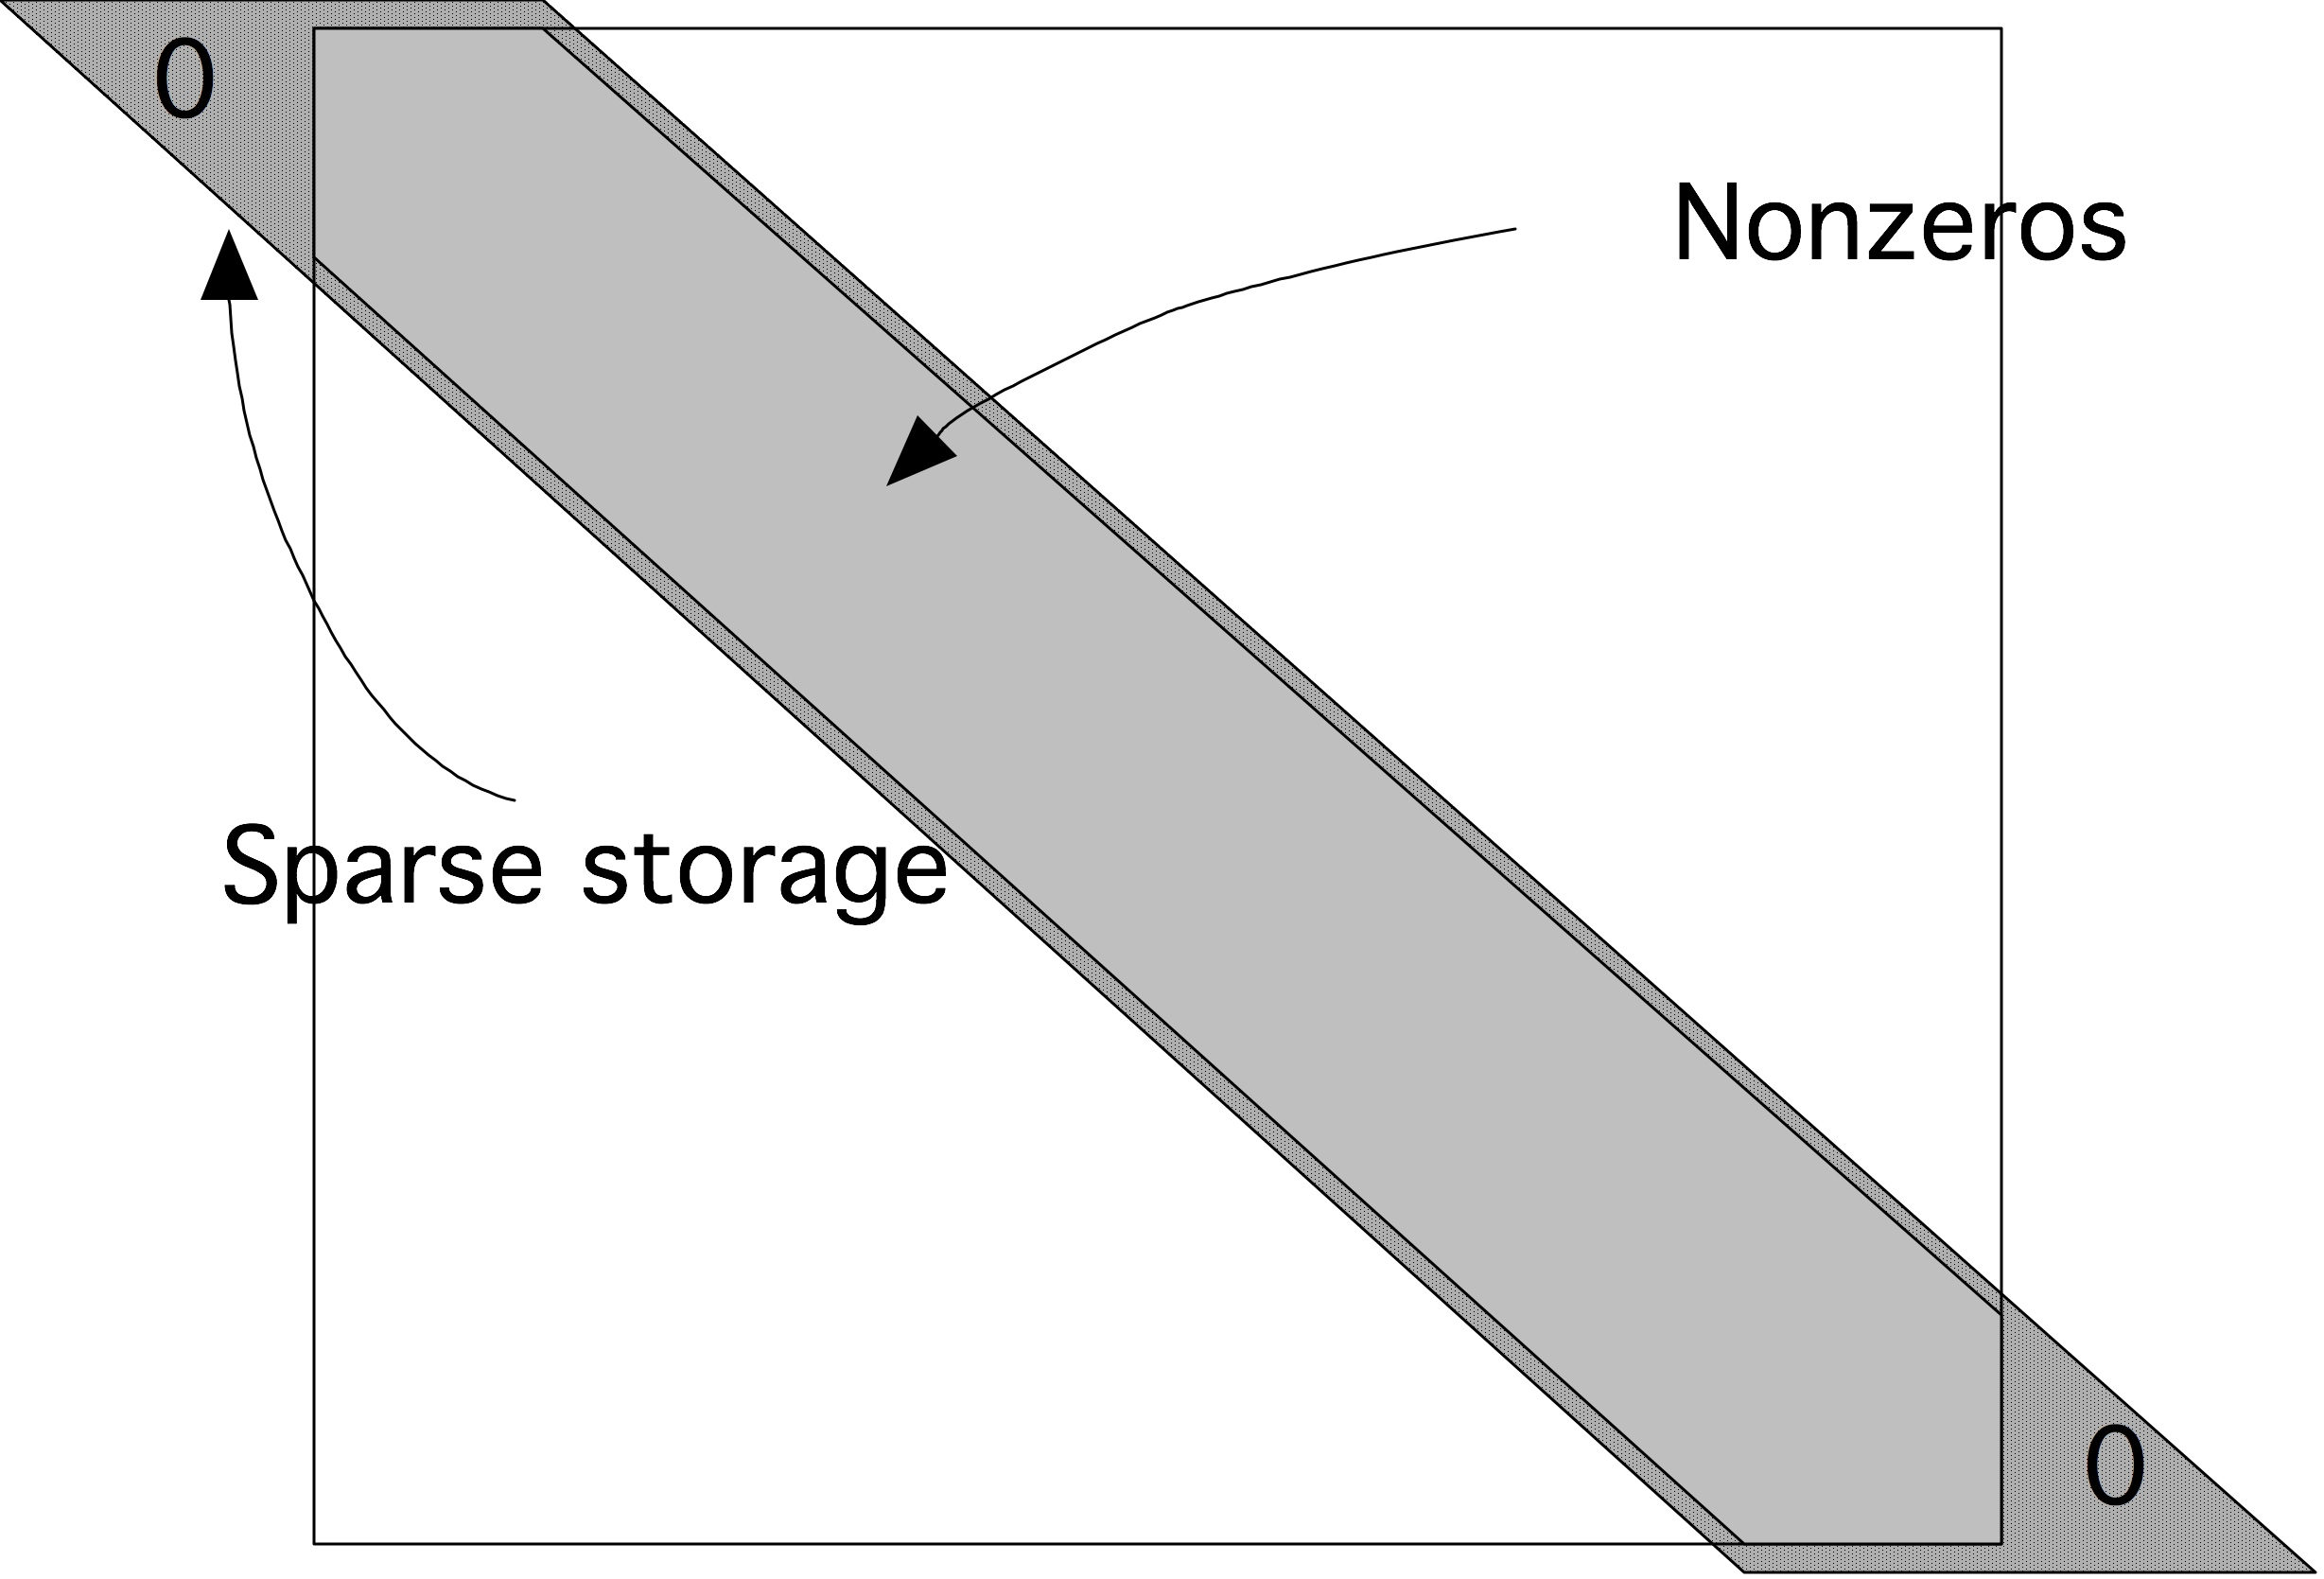
\includegraphics[scale=.1]{sparsediag}
  \end{frame}

  \begin{frame}[fragile]{Diagonal matrix-vector product}
    \[ y_i \leftarrow y_i + A_{ii} x_i, \]
    \[ y_i \leftarrow y_i + A_{ii+1} x_{i+1}\quad\hbox{for $i<n$}, \]
    \[ y_i \leftarrow y_i + A_{ii-1} x_{i-1}\quad\hbox{for $i>1$}. \]

\begin{verbatim}
for diag = -diag_left, diag_right
    for loc = max(1,1-diag), min(n,n-diag)
        y(loc) = y(loc) + val(loc,diag) * x(loc+diag)
    end
end
\end{verbatim}
  \end{frame}

  \begin{frame}{Pro/con}
    Pro: long vectors (D'Azevedo: $20\times$ speedup on Cray X-1)

    Con: limited, little cache reuse

    Variants: jagged diagonal
  \end{frame}

  \begin{frame}{Jagged diagonal storage}
    Align irregular sparse matrices along `jagged' diagonals

    \[
    \begin{pmatrix}
      10&-3&0&1&0&0\\ 0&9&6&0&-2&0\\ 3&0&8&7&0&0\\
      0&6&0&7&5&4\\ 0&0&0&0&9&13\\ 0&0&0&0&5&-1
    \end{pmatrix}
    \rightarrow
    \begin{pmatrix}
      10&-3&1\\ 9&6&-2\\ 3&8&7\\
      6&7&5&4\\ 9&13\\ 5&-1
    \end{pmatrix}
    \]
    %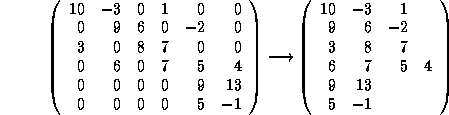
\includegraphics[scale=.6]{jagged}
  \end{frame}

  \begin{frame}
    Long vectors make it suitable for GPU

    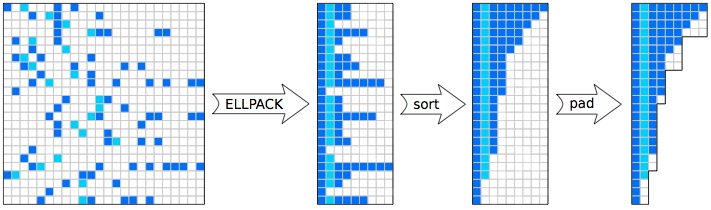
\includegraphics[scale=.45]{padded-elpack}
  \end{frame}
\end{diagonalstorage}

\frame{\frametitle{Fill-in}
  Remember Gaussian elimination algorithm:
\begin{tabbing}
  \kern20pt\=\kern10pt\=\kern10pt\=\kern10pt\=\kill
  \>for\={} $k=1,n-1$:\\
  \>\>for\={} $i=k+1$ to $n$:\\
  \>\>\>for\={} $j=k+1$ to $n$:\\
  \>\>\>\>$a_{ij}\leftarrow a_{ij}-a_{ik}*a_{kj}/a_{kk}$
\end{tabbing}
  
Fill-in: index $(i,j)$ where $a_{ij}=0$ originally,
but gets updated to non-zero.\\
(and so $\ell_{ij}\not=0$ or $u_{ij}\not=0$.)

Change in the sparsity structure! How do you deal with that?
}

\begin{frame}{LU of a sparse matrix}
\[
\begin{pmatrix}
  2&-1&0&\ldots\\ -1&2&-1\\ 0&-1&2&-1\\ 
  &\ddots&\ddots&\ddots&\ddots
\end{pmatrix}
\quad\Rightarrow\quad
\left(\begin{array}{c|cccc}
  2&-1&0&\ldots\\ \hline 0&2-\frac12&-1\\ 0&-1&2&-1\\ 
  &\ddots&\ddots&\ddots&\ddots
\end{array}\right)
\]
How does this continue by induction?

Observations?
\end{frame}

\frame{\frametitle{LU of a sparse matrix}
\small
\[
\left(\begin{array}{ccccc:cccc}
  4&-1&0&\ldots&&-1\\ -1&4&-1&0&\ldots&0&-1\\ 
  &\ddots&\ddots&\ddots&&&\ddots\\ \hdashline
  -1&0&\ldots&&&4&-1\\ 0&-1&0&\ldots&&-1&4&-1\\
\end{array}\right)
\] \[
\Rightarrow\quad
\left(\begin{array}{c|cccc:cccc}
  4&-1&0&\ldots&&-1\\ \hline &4-\frac14&-1&0&\ldots&-1/4&-1\\ 
  &\ddots&\ddots&\ddots&&&\ddots\\ \hdashline
  &-1/4&\ldots&&&4-\frac14&-1\\ &-1&0&\ldots&&-1&4&-1\\
\end{array}\right)
\]
}

\begin{frame}{A little graph theory}
  Graph is a tuple $G=\langle V,E\rangle$ where
  $V=\{v_1,\ldots v_n\}$ for some~$n$, and $E\subset\{(i,j)\colon 1\leq
  i,j\leq n,\,i\not=j\}$.

  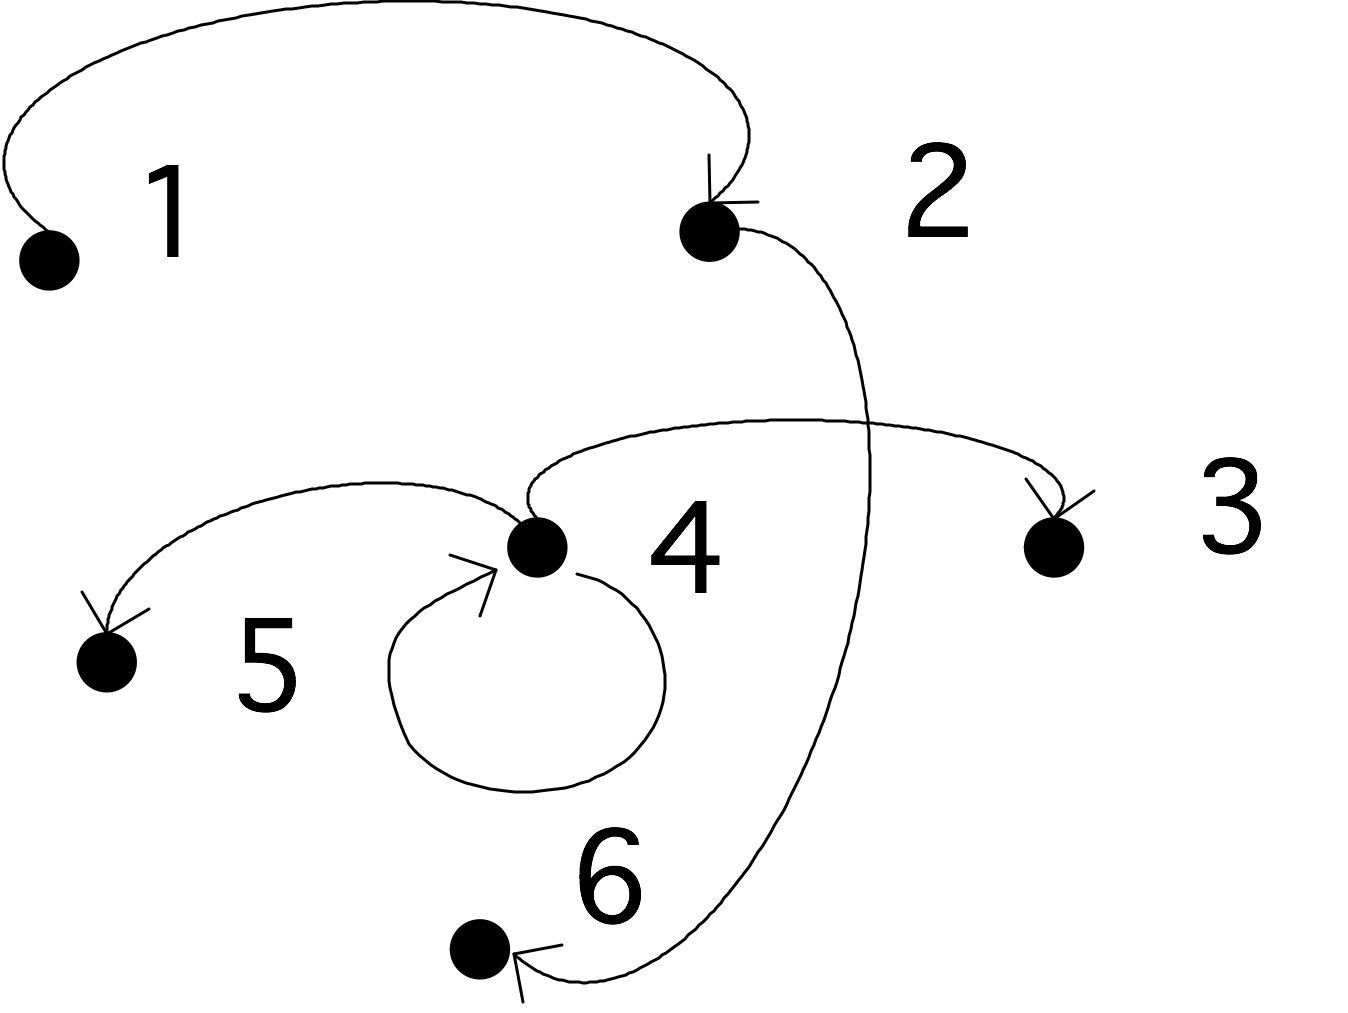
\includegraphics[scale=.1]{graph1}

  \[    \begin{cases}
    V=\{1,2,3,4,5,6\}\\
    E=\{ (1,2),(2,6),(4,3),(4,4),(4,5)\}
  \end{cases}
  \]
\end{frame}

\begin{frame}{Graphs and matrices}
  For a graph $G=\langle V,E\rangle$,
  the adjacency matrix $M$ is defined by
  \[ 
  M_{ij}=
  \begin{cases}1&(i,j)\in E\\ 0&\mbox{otherwise}\end{cases}
  \]
  
  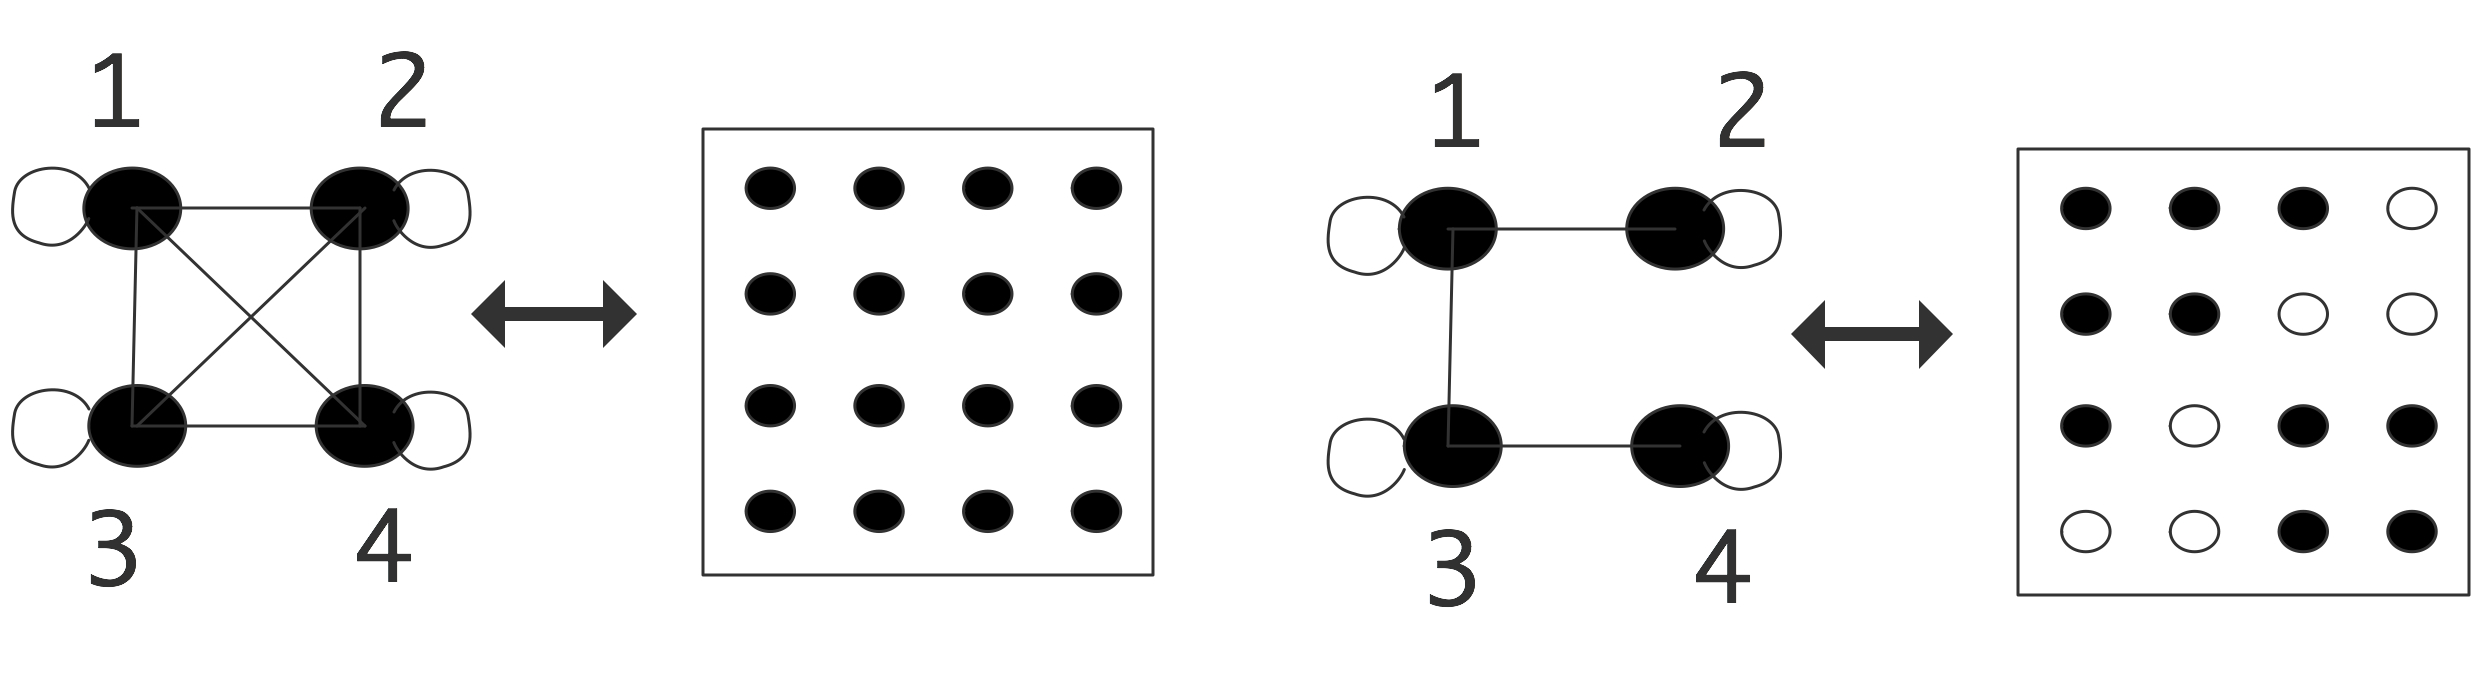
\includegraphics[scale=.11]{matrix-graph}

  A dense and a sparse matrix, both with their adjacency
  graph
\end{frame}

\frame{\frametitle{Fill-in}
  Fill-in: index $(i,j)$ where $a_{ij}=0$ originally,
  but gets updated to non-zero.

  \[ a_{ij}\leftarrow a_{ij}-a_{ik}*a_{kj}/a_{kk} \]


  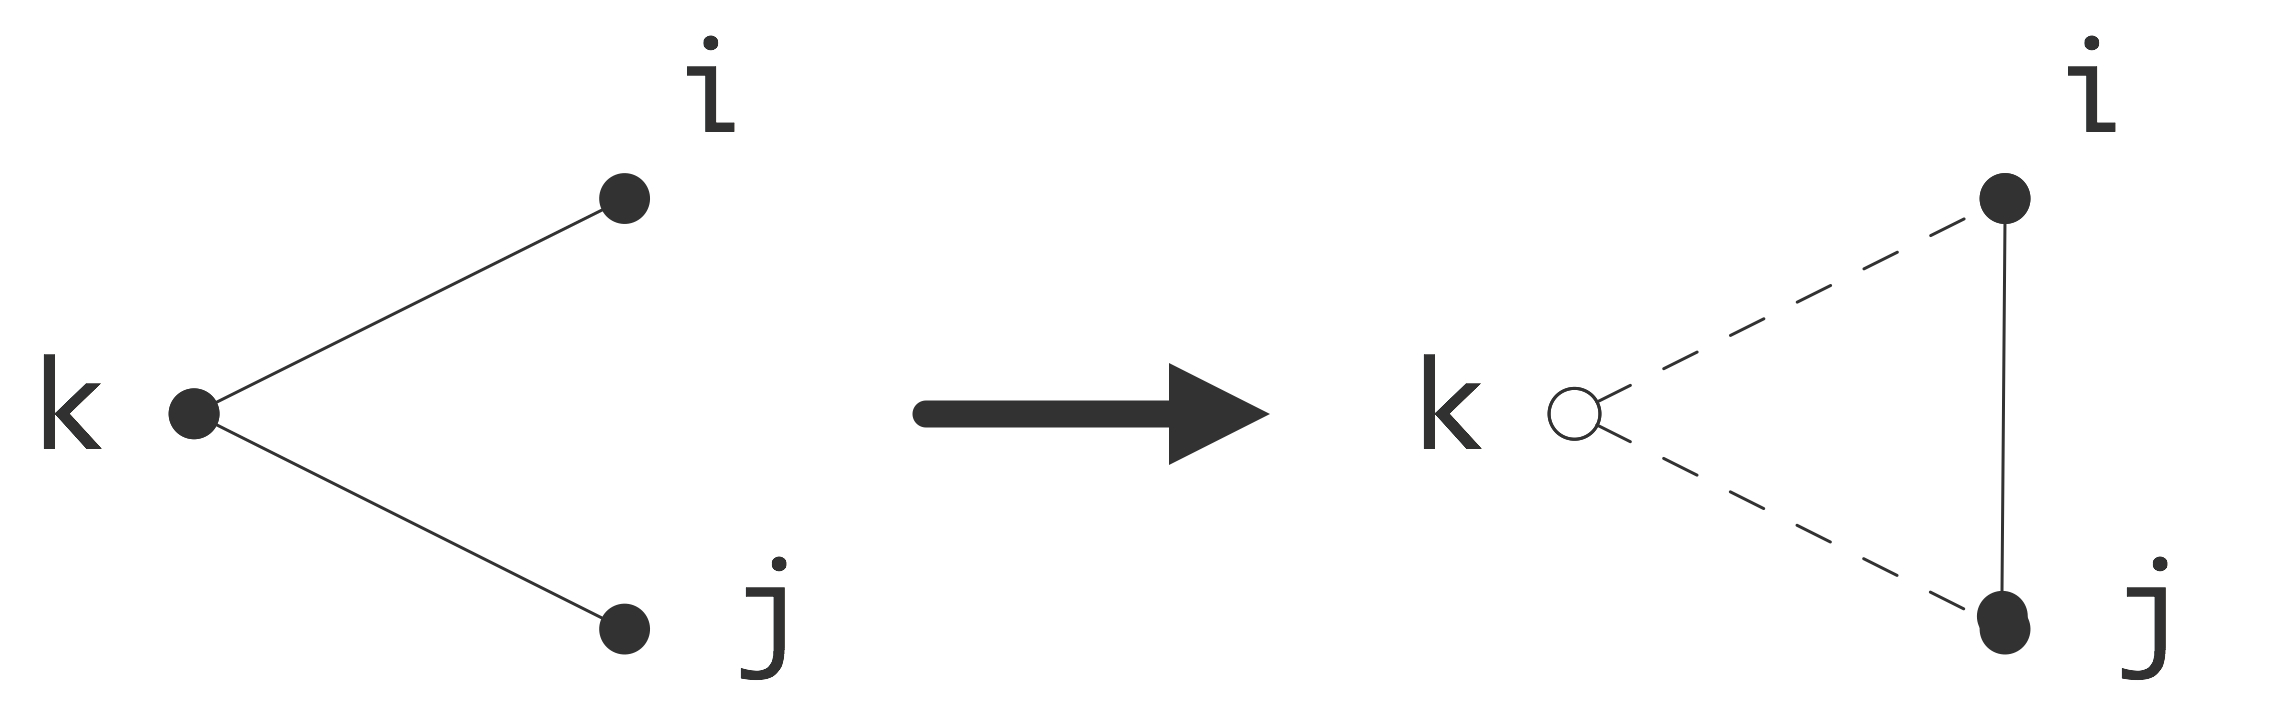
\includegraphics[scale=.12]{ijk-eliminate}

  Eliminating a vertex introduces a new edge in the quotient
    graph
}

\begin{frame}{LU of sparse matrix, with graph view: 1}
Original matrix.\\
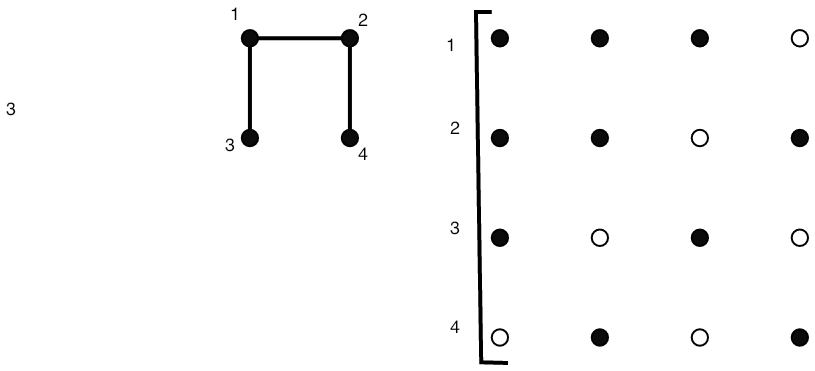
\includegraphics[scale=.25]{gaussgraph1}
\end{frame}
\begin{frame}{LU of sparse matrix, with graph view: 2}
  Eliminating $(2,1)$ causes fill-in at $(2,3)$.\\
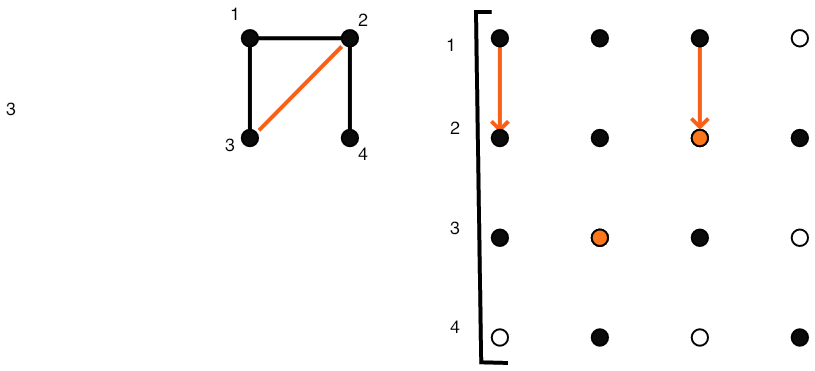
\includegraphics[scale=.25]{gaussgraph2}
\end{frame}
\begin{frame}{LU of sparse matrix, with graph view: 3}
  Remaining matrix when step~1 finished.\\
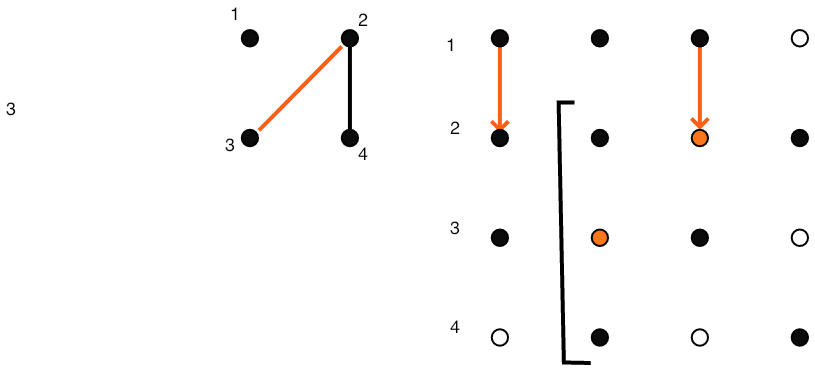
\includegraphics[scale=.25]{gaussgraph3}
\end{frame}
\begin{frame}{LU of sparse matrix, with graph view: 4}
  Eliminating $(3,2)$ fills $(3,4)$\\
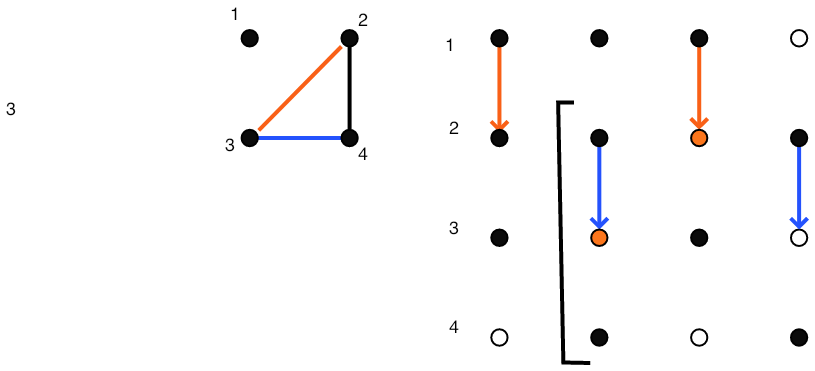
\includegraphics[scale=.25]{gaussgraph4}
\end{frame}
\begin{frame}{LU of sparse matrix, with graph view: 5}
  After step~2\\
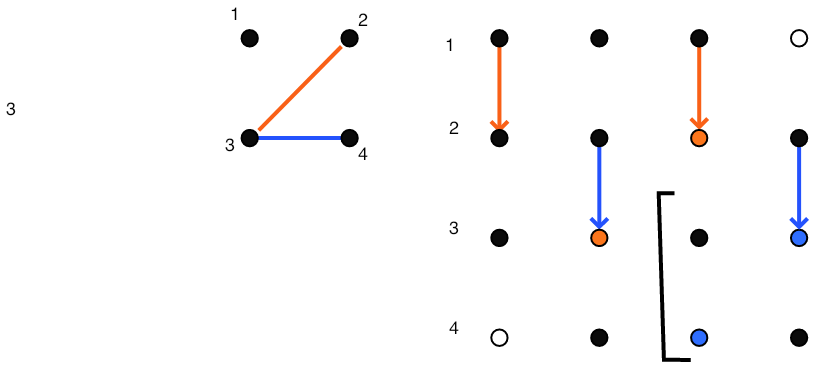
\includegraphics[scale=.25]{gaussgraph5}
\end{frame}

\frame{\frametitle{Fill-in is a function of ordering}
  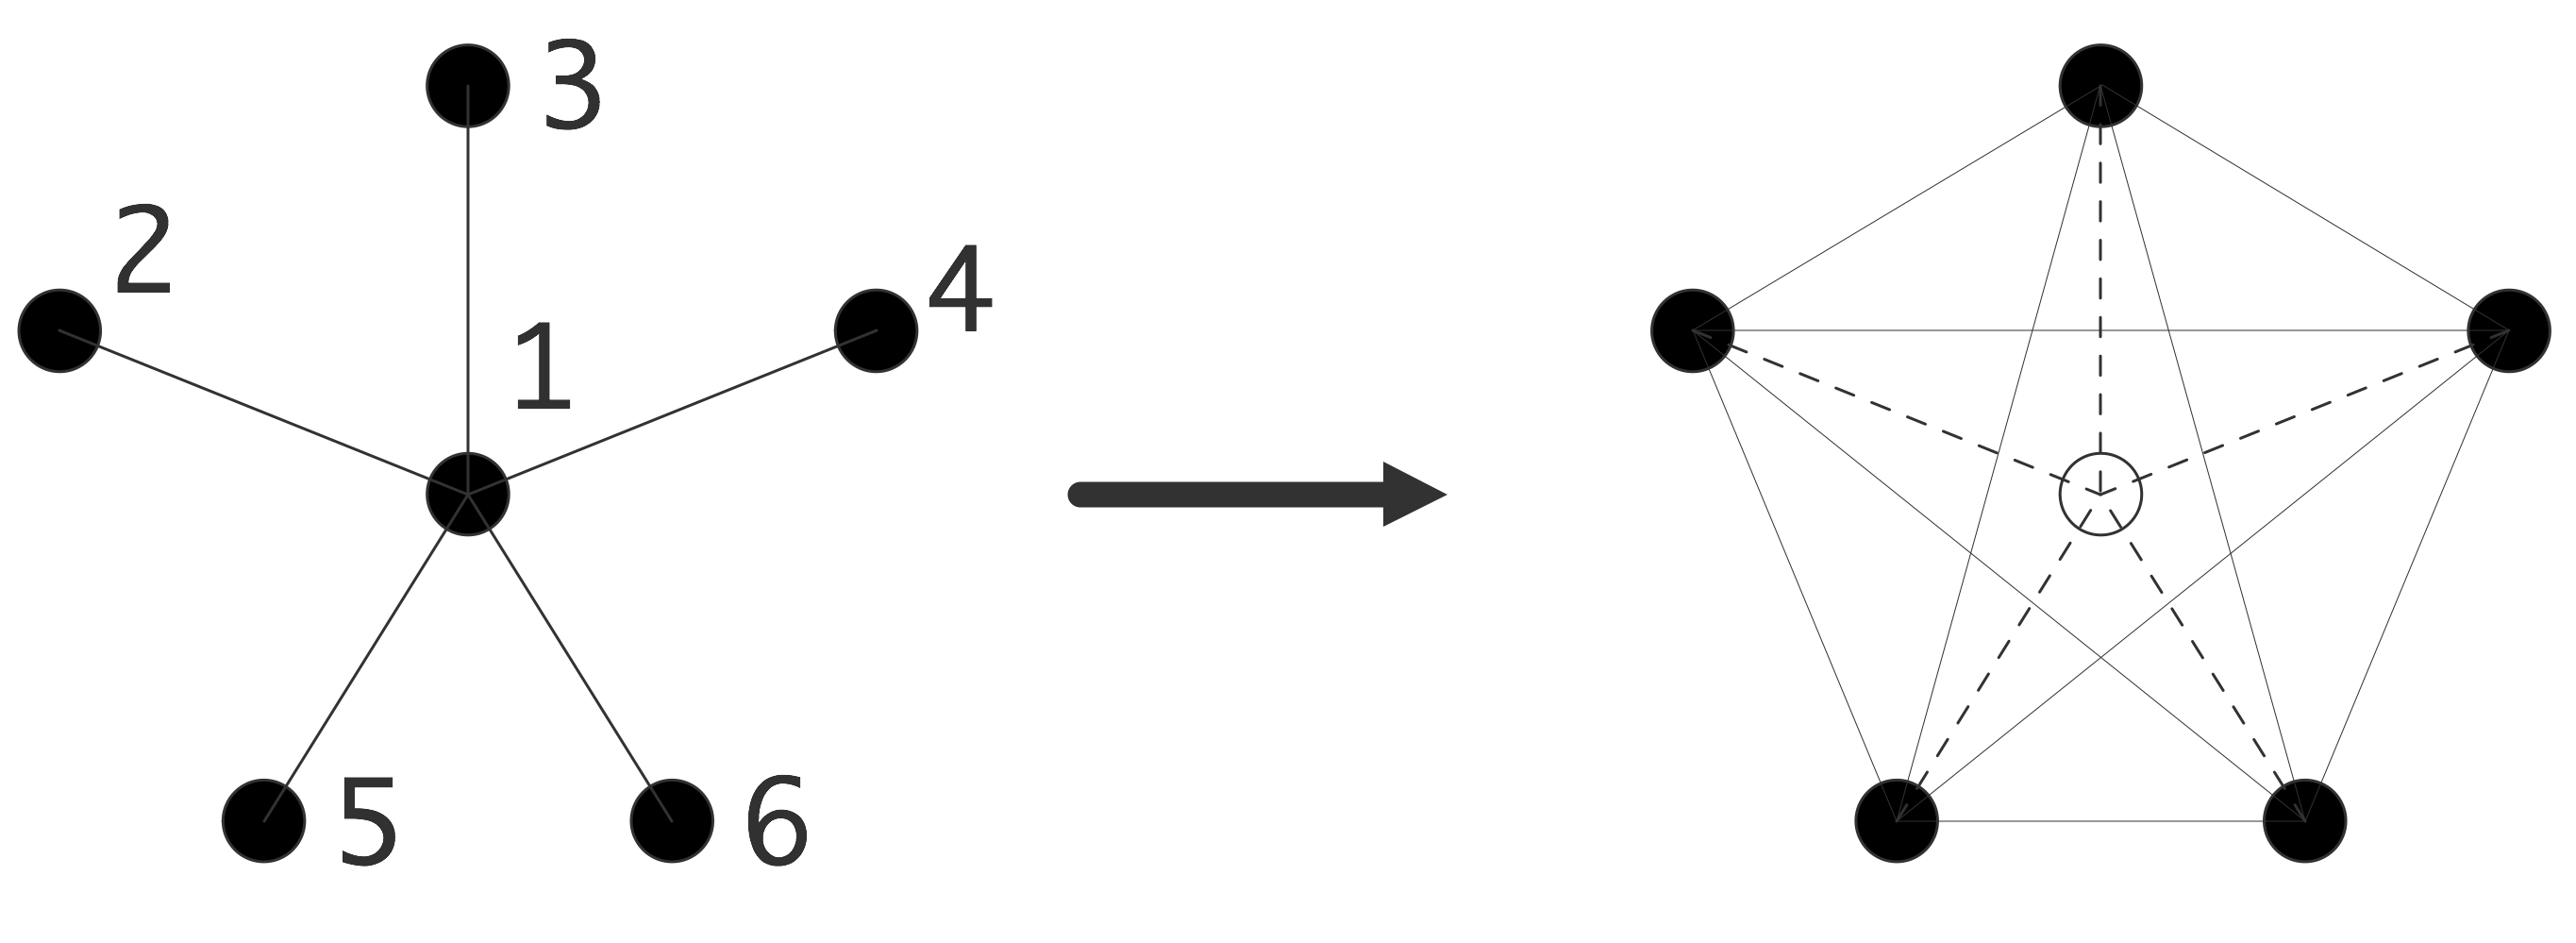
\includegraphics[scale=.1]{starmatrix}
  \[ 
  \begin{pmatrix}
    *&*&\cdots&*\\ *&*&&\emptyset\\ \vdots&&\ddots\\ *&\emptyset&&*
  \end{pmatrix}
  \]
  After factorization the matrix is dense.\\
  Can this be permuted?
}

\begin{frame}{Exercise: LU of a penta-diagonal matrix}
  Consider the matrix
  \[
  \begin{pmatrix}
    2&0&-1\\
    0&2&0&-1\\
    -1&0&2&0&-1\\
    &-1&0&2&0&-1\\
    &&\ddots&\ddots&\ddots&\ddots&\ddots\\
  \end{pmatrix}
  \]
  Describe the $LU$ factorization of this matrix:
  \begin{itemize}
  \item Convince yourself that there will be no fill-in. Give an inductive proof of this.
  \item What does the graph of this matrix look like?
    (Find a tutorial on graph theory. What is a name for such a graph?)
  \item Can you relate this graph to the answer on the question of the fill-in?
  \end{itemize}
\end{frame}

\begin{frame}{Exercise: LU of a band matrix}
  Suppose a matrix $A$ is banded with \emph{halfbandwidth}~$p$:
  \[ a_{ij}=0\quad\hbox{if $|i-j|>p$} \]
  Derive how much space an LU factorization of~$A$ will take if no
  pivoting is used. (For bonus points: consider partial pivoting.)

  Can you also derive how much space the inverse will take? (Hint: if
  $A=LU$, does that give you an easy formula for the inverse?)
\end{frame}

\endinput 

%%%%
%%%% graph theory stuff
%%%%

\frame{\frametitle{Graph theory of sparse matrices}
  Some things (reducibility) are easiest seen in a graph
  
  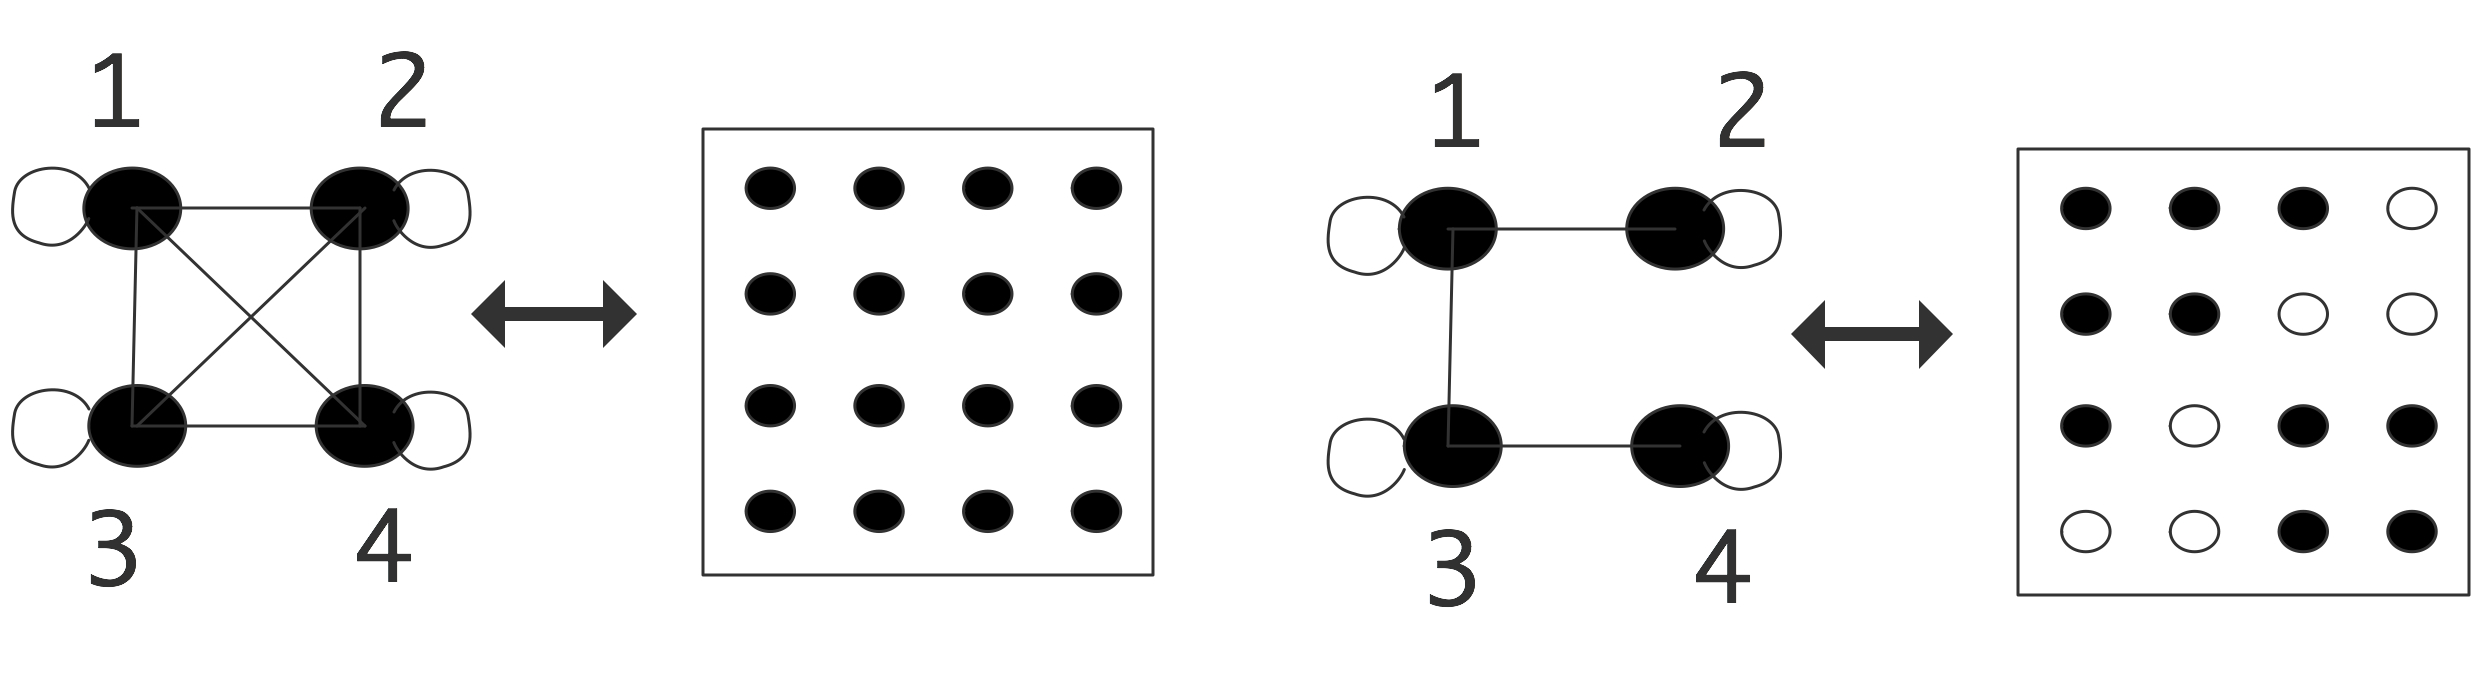
\includegraphics[scale=.12]{matrix-graph}
}

\frame{\frametitle{Graph theory of sparse elimination}
  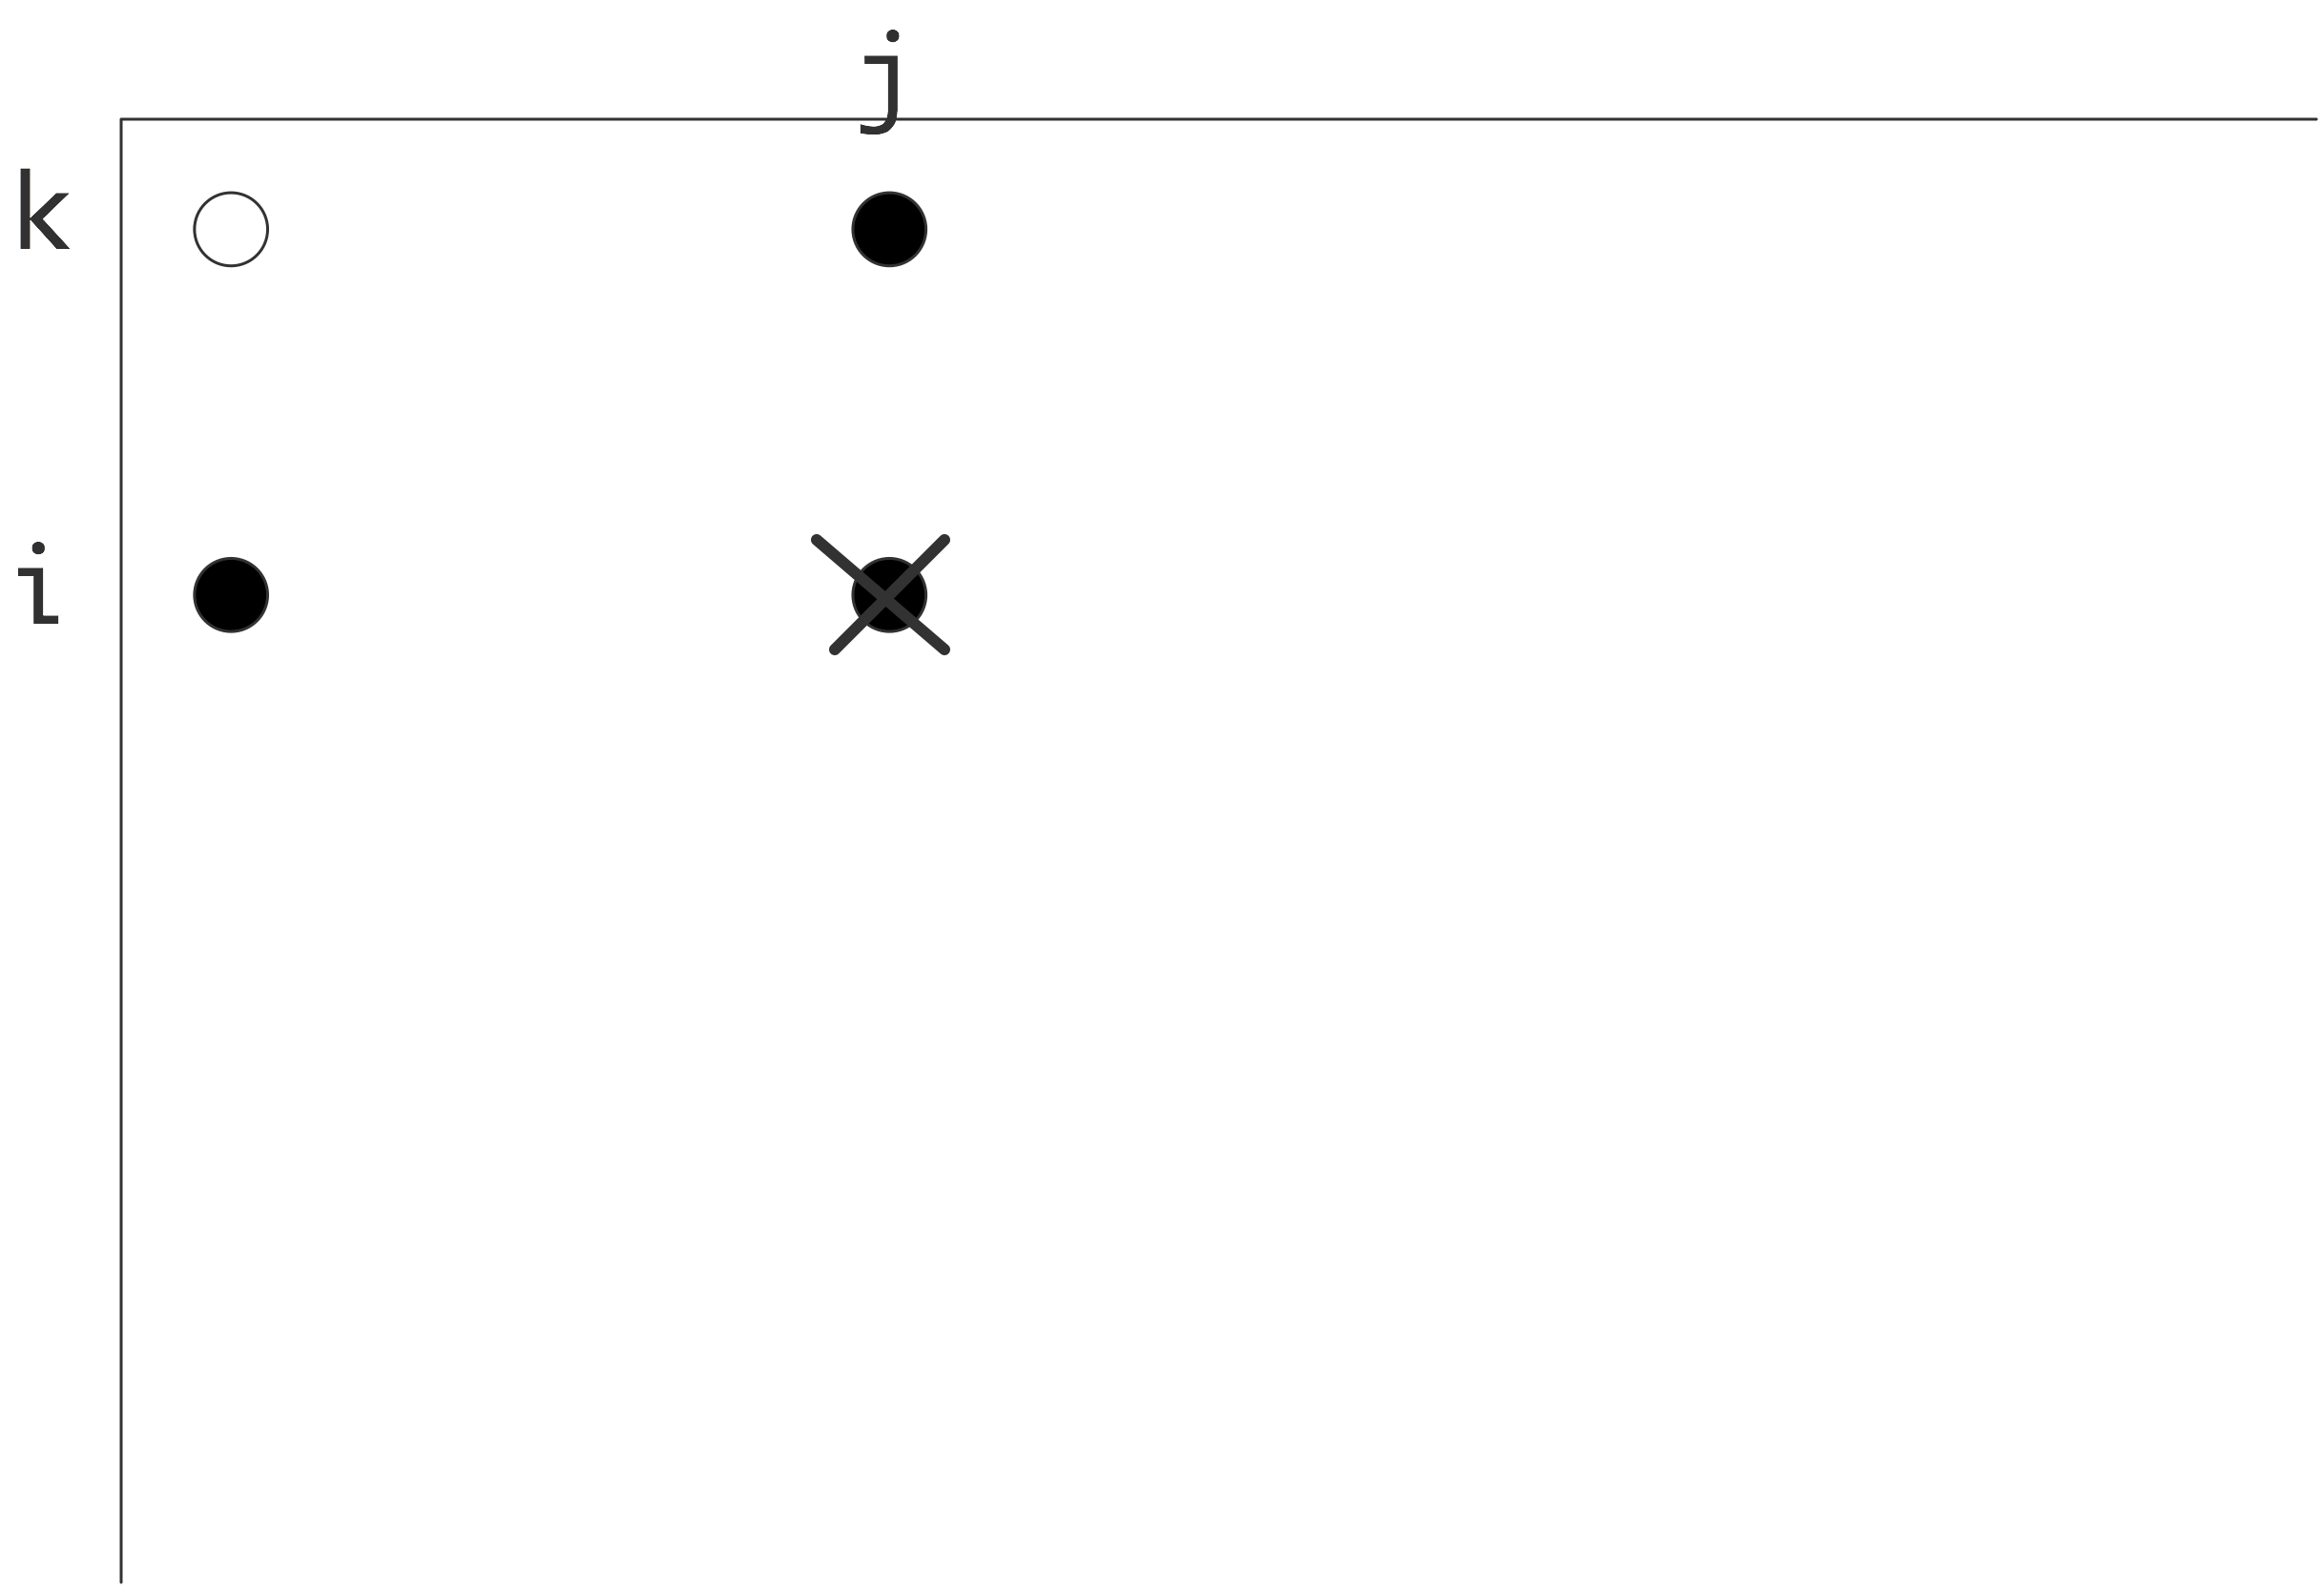
\includegraphics[scale=.06]{ijk-matrix-eliminate}
$a_{ij} \leftarrow a_{ij}- a_{ik}a_{kk}\inv a_{kj}$

  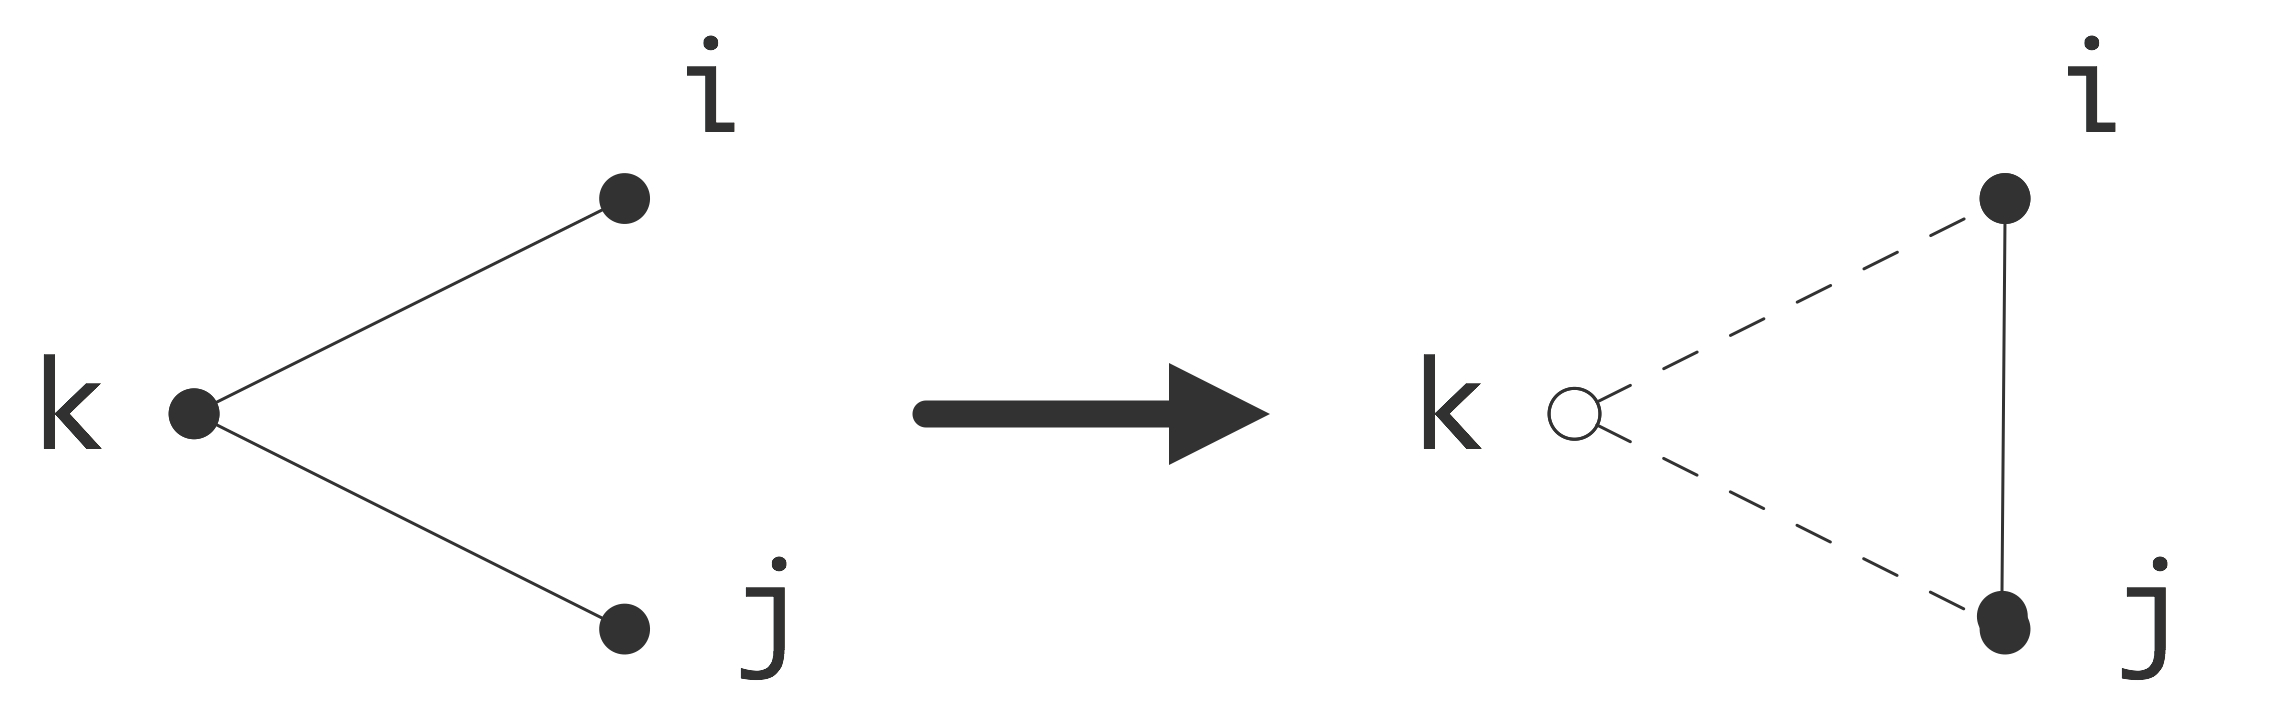
\includegraphics[scale=.1]{ijk-eliminate}
}

\begin{frame}{Domain view}
Graph of connectivity of variables:

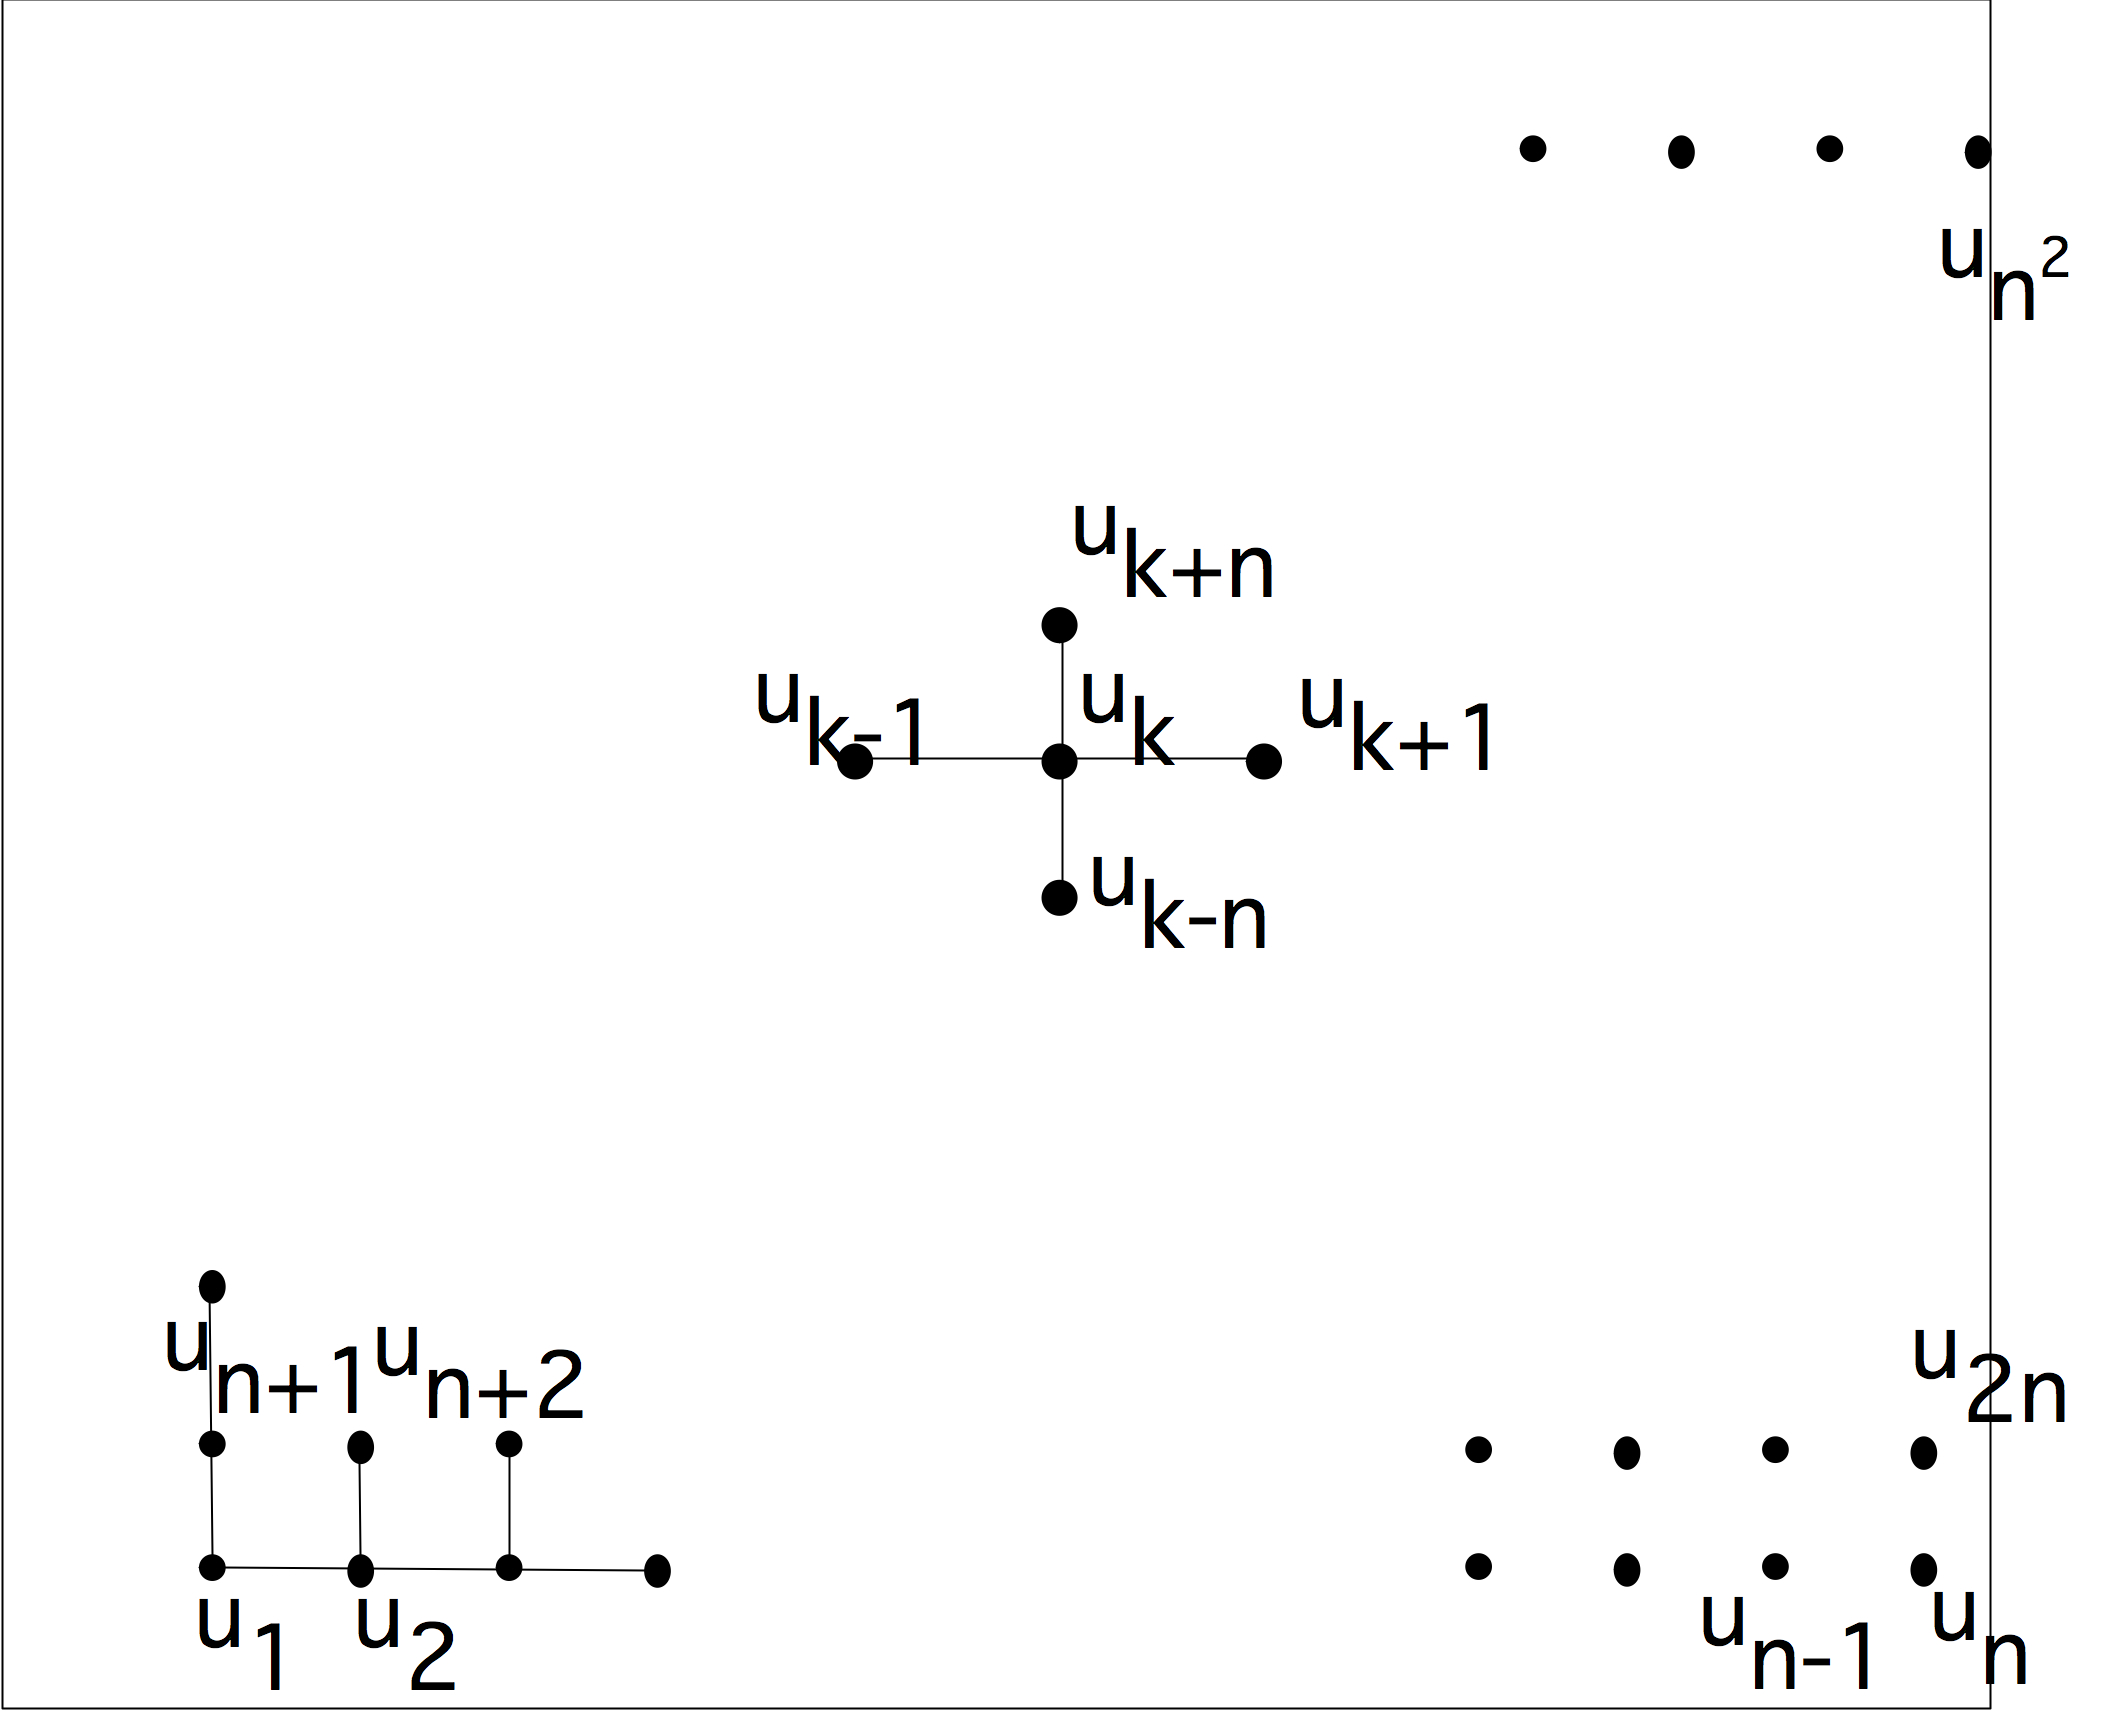
\includegraphics[scale=.07]{laplacedomain-connect}

now start eliminating in sequence
\end{frame}

\frame{
  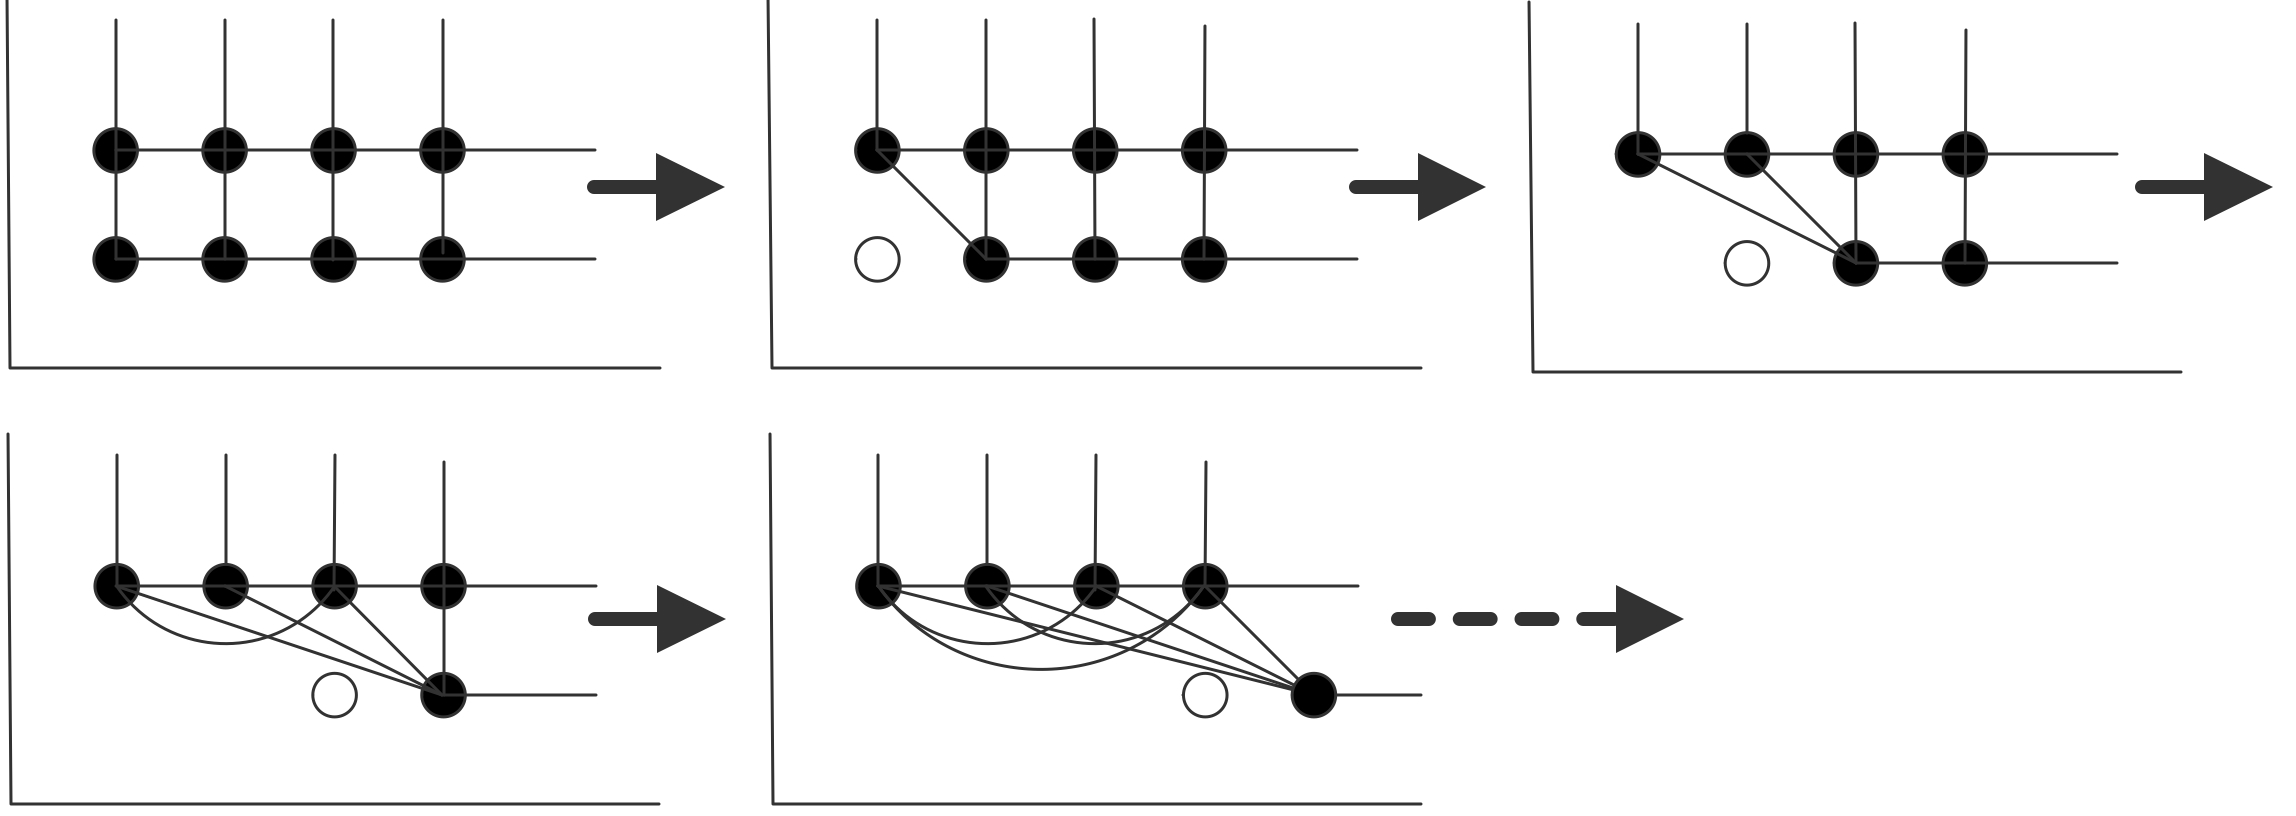
\includegraphics[scale=.15]{row-eliminate}

Remaining matrix has a dense leading block
}

\frame{\frametitle{Fill-in during LU}
Recall:

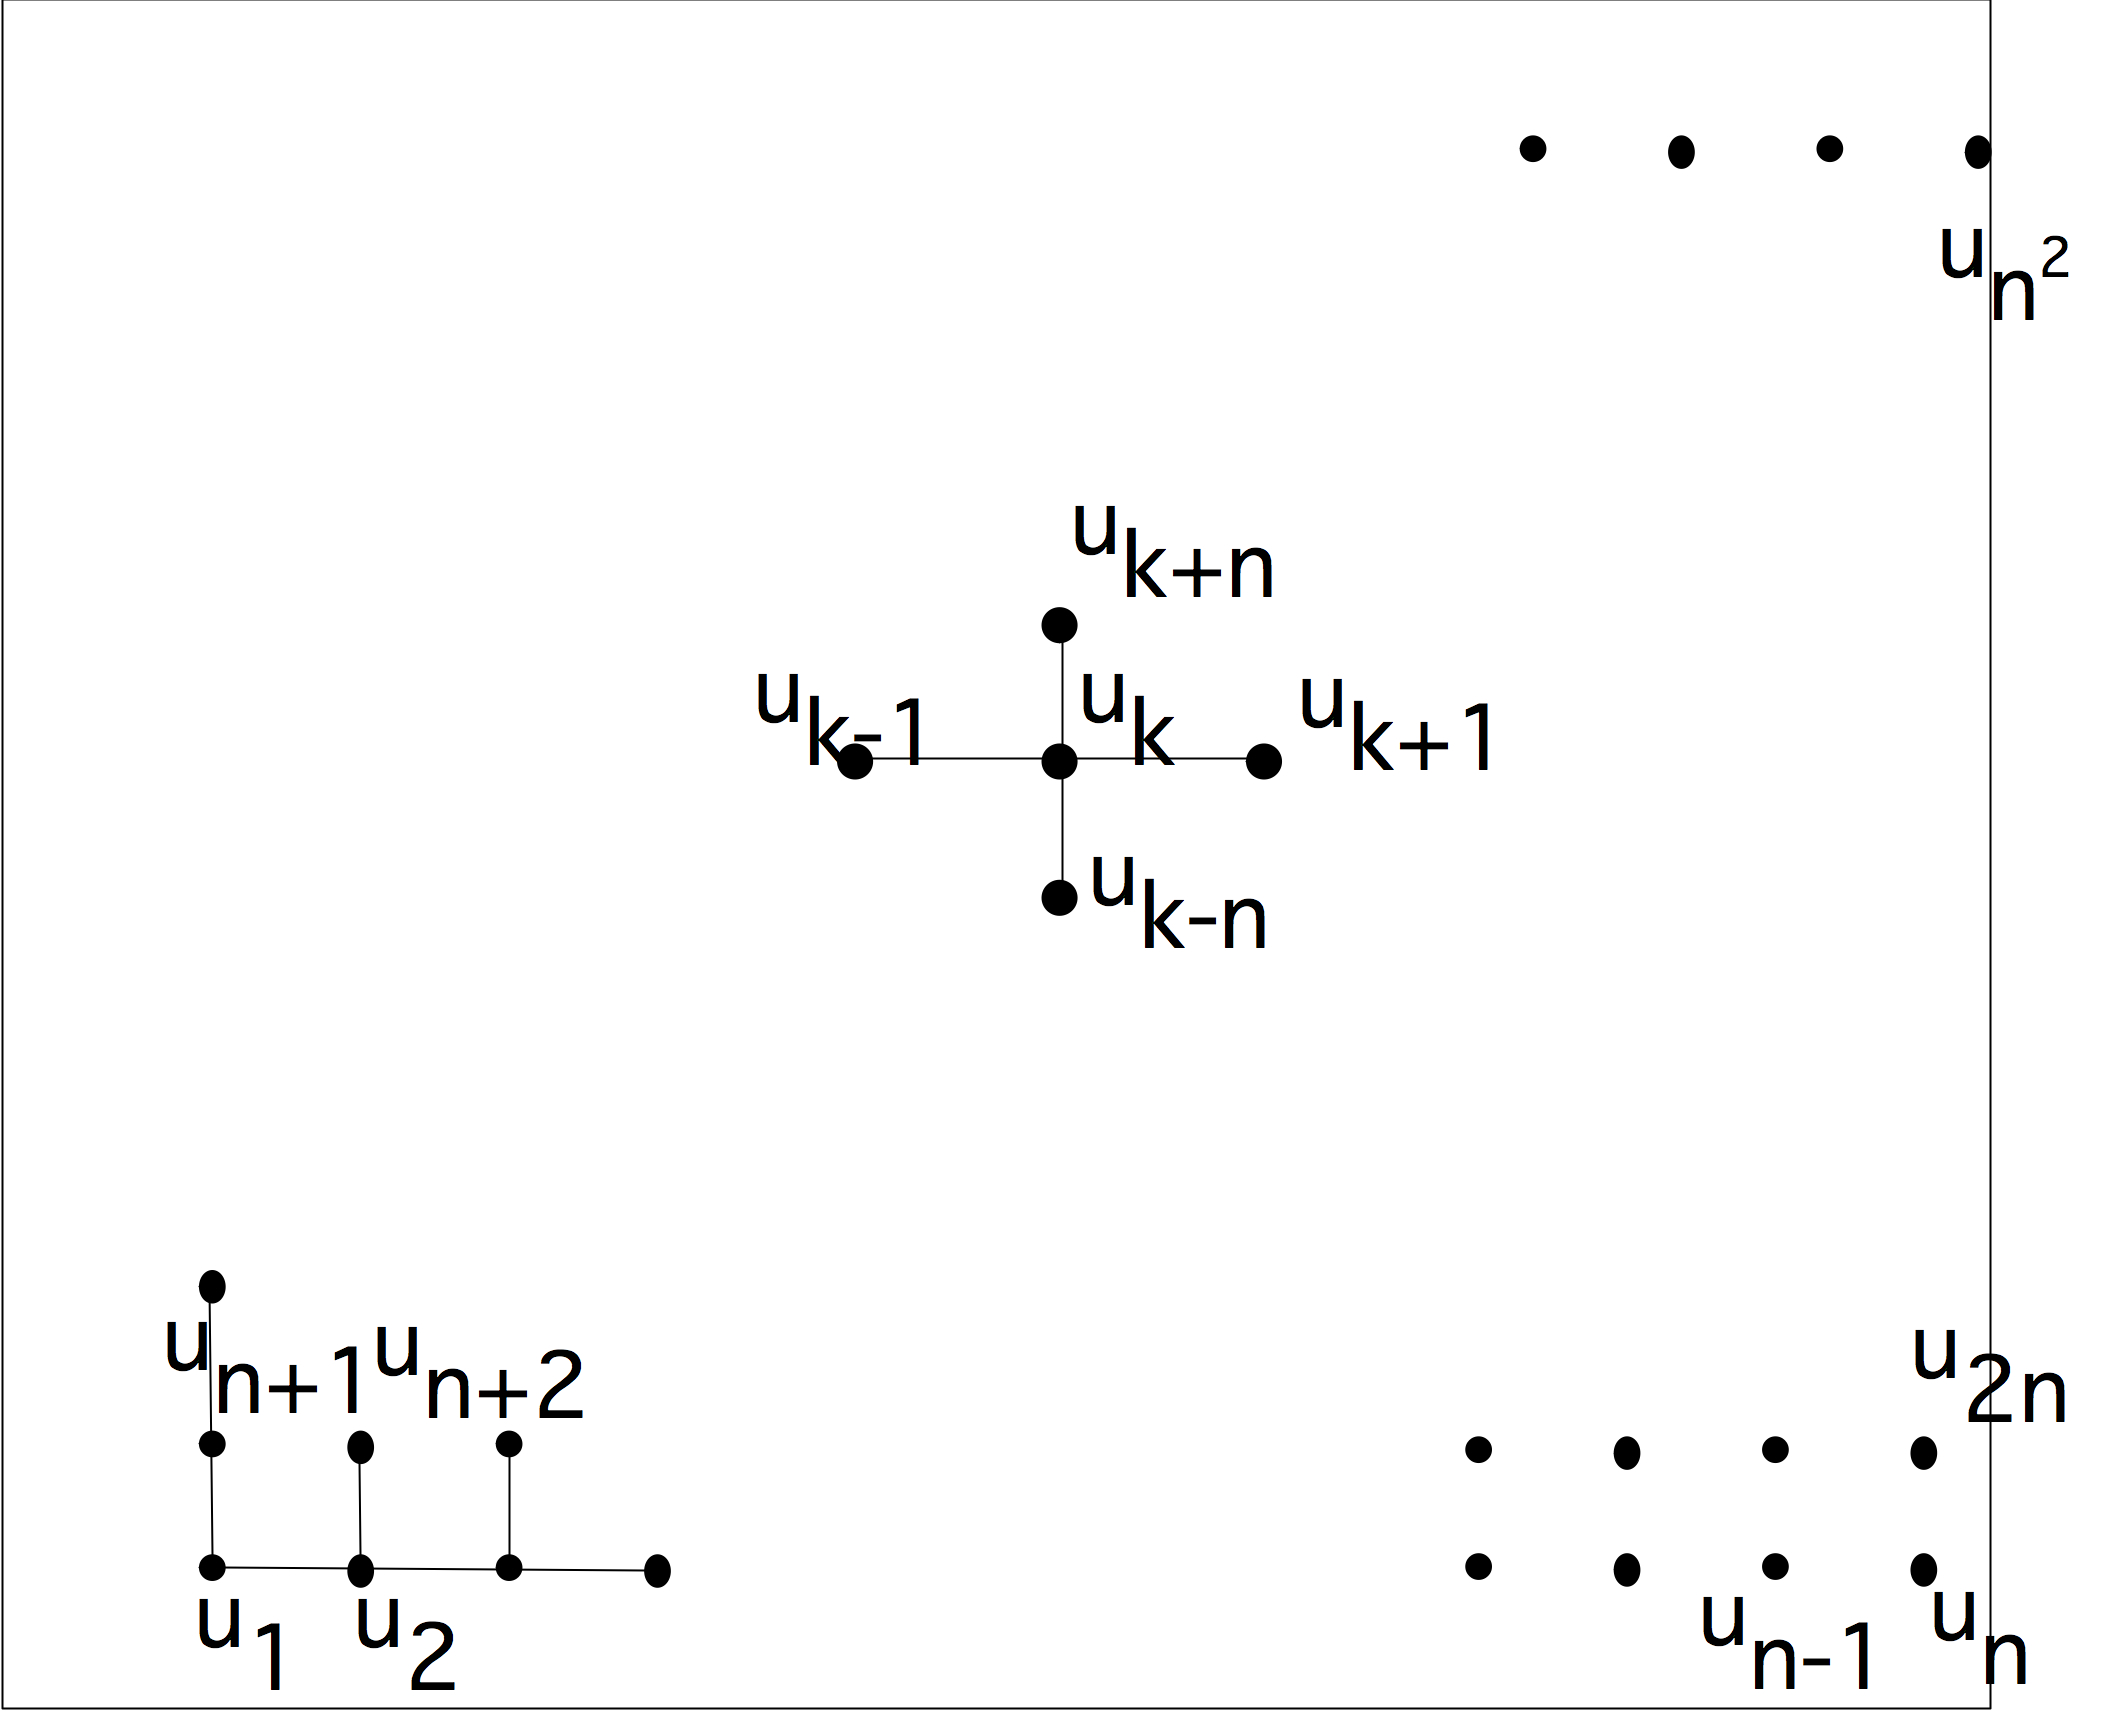
\includegraphics[scale=.07]{laplacedomain-connect}
}

\frame{\frametitle{Fill-in during LU}

2D BVP: $\Omega$ is $n\times n$, gives matrix of size $N=n^2$, with
bandwidth~$n$. 

Matrix storage $O(N)$

LU storage $O(N^{3/2})$ (limited to band)

LU factorization work $O(N^2)$

Cute fact: storage can be computed linear in \#nonzeros
}

\endinput
\frame{\frametitle{Fill-in is a function of ordering}

  \[ 
  \begin{pmatrix}
    *&*&\cdots&*\\ *&*&&\emptyset\\ \vdots&&\ddots\\ *&\emptyset&&*
  \end{pmatrix}
  \]
  After factorization the matrix is dense.\\
  Can this be permuted?
}

